\clearpage
\singlespacing
\renewcommand\thesubsection{\Roman{subsection}}
\counterwithin{figure}{section}
\counterwithin{table}{section}
\setcounter{page}{1}
\appendices
\subsubsection*{Women Also Know Stuff: Challenging the Gender Gap in Political Sophistication}
\startcontents[sections]
\printcontents[sections]{l}{1}{\setcounter{tocdepth}{2}}
\thispagestyle{empty}
\clearpage
\newpage\setcounter{page}{1}

\section{Data Overview}\label{app:variables}

\subsection{Open-Ended Items}

\paragraph{2018 Cooperative Election Study (CES):}
The main analysis focuses on a national stratified survey of 1,000 respondents as part of the 2018 CES. Among other items, the study includes the following open-ended questions:
\begin{itemize}
	\item On the issue of \textbf{gun legislation}, please outline the main arguments that come to mind \textit{in favor and against} background checks for all gun sales, including at gun shows and over the Internet.
	\item On the issue of \textbf{abortion}, please outline the main arguments that come to mind \textit{in favor and against} banning abortions after the 20th week of pregnancy.
	\item On the issue of \textbf{immigration}, please outline the main arguments that come to mind \textit{in favor and against} providing a legal status for recipients of the Deferred Action for Childhood Arrivals (DACA) status.
	\item On the issue of \textbf{health cure}, please outline the main arguments that come to mind \textit{in favor and against} repealing the Affordable Care Act (Obamacare).
	\item On the issue of \textbf{trade policies}, please outline the main arguments that come to mind \textit{in favor and against} imposing tariffs on imported steel and aluminum from countries including Canada, Europe, and Mexico.
\end{itemize}

\paragraph{2020, 2016, \& 2012 American National Election Study (ANES):}
In addition to the original data collection as part of the CES, I apply the measurement approach using three separate waves of the American National Election Study (ANES), each of which consists of a representative survey of about 5000 adults in the months before the US Presidential election in each year. Here, discursive sophistication is evaluated using a set of 8 open-ended questions in which respondents were asked to list anything in particular that they like/dislike about the Democratic/Republican party as well as anything that might make them vote/not vote for either of the Presidential candidates.

% TODO: add footnote again after reviews
\paragraph{2015 YouGov Survey}
In order to replicate and extend the main analysis, I rely on a separate nationally representative survey employing yet another alternative set of open-ended responses. The data was collected by YouGov in December 2015 and contains responses of 1000 U.S. residents. %\footnote{See \citet{clifford2018disgust} for details on the study.} 
As part of this study, respondents were asked to describe their attitudes towards two prominent political issues that were discussed frequently in the media. First, they were asked in a closed format whether they favor or oppose stricter gun laws. Subsequently, they were asked to respond to the following two questions:
\begin{itemize}\setlength\itemsep{0em}
	\item Still thinking about the question you just answered, what thoughts came to mind while you were answering that question? Please try to list everything that came to mind.
	\item Thinking about the mass shootings that have occurred in the U.S. in the last few years, what factors do you think are responsible for the shootings?
\end{itemize}
Second, the respondents reported on their attitudes towards the Affordable Care Act in a closed format and were then asked to elaborate in their own words by answering the following questions:
\begin{itemize}\setlength\itemsep{0em}
	\item Still thinking about the question you just answered, what thoughts came to mind while you were answering that question? Please try to list everything that came to mind.
	\item For decades, experts have observed that the United States spends far more per person on health care than any other country. However, the U.S. falls behind on most measures of health care outcomes, such as life expectancy. What factors do you think are responsible for the state of our health care system?
\end{itemize}
%Here, discursive sophistication is evaluated based on the verbatim responses to the four preceding questions using the same procedures described above. 
%Similar to the CES study, the questions directly address considerations related to specific policy issues that were prominent in the political discourse at the time of the survey.

\paragraph{Swiss Referendum Survey}
Lastly, I examine survey data on Swiss citizens justifying their vote choices on multiple referenda used in a recent analysis by \citet{colombo2016justifications}. The author compiled a data set of cross-sectional surveys administered in Switzerland after national popular votes on multiple policy propositions. The original surveys were conducted as representative samples after each of thirty-four national policy votes that were held between 2008 and 2012 resulting in a total of about 27,000 observations. Respondents who participated in a given referendum (ca. 22,000 in total) were asked to describe the main reason as well as additional justifications for their decision in two separate items. 
%As before, discursive sophistication is evaluated based on verbatim responses to both questions. Since the Swiss survey was conducted in three different languages (German, French, and Italian), I computed the measure of discursive sophistication separately for each group of respondents.
% QUESTION wording for Swiss study?


%\clearpage
\subsection{Conventional Knowledge Items}

\begin{itemize}
	\item \textit{2018 CES}: Additive index containing 5 items (gun legislation, trade policy, DACA, health care, abortion).
	\item \textit{2020 ANES}: Additive index containing 4 items (length of Senate term, federal government spending, majority in House, majority in Senate).
	\item \textit{2016 ANES}: Additive index containing 4 items (length of Senate term, federal government spending, majority in House, majority in Senate). %`Don't know' responses are considered incorrect. Interviewer evaluations are based on the assessment of the respondent's general level of information about politics recorded at the end of the pre-election wave.	
	\item \textit{2012 ANES}: Additive index containing 5 items (number of Presidential terms, size of budget deficit, length of Senate term, meaning of Medicare, federal government spending). %`Don't know' responses are considered incorrect. Interviewer evaluations are based on the assessment of the respondent's general level of information about politics recorded at the end of the pre-election wave.
	\item \textit{2015 YouGov}: Additive index containing 8 items (Speaker of the House, meaning of TPP, Chair of Federal Reserve Board, current unemployment rate, Presidential veto override, meaning of Common Core, leading source of electricity in US, majority in Senate). %`Don't know' responses are considered incorrect.
\end{itemize}

%\paragraph{Dependent variables:}
%\begin{itemize}
%	\item \textit{Turnout}: Dichotomous indicator.
%	\item \textit{Political Interest}: 
%	\item \textit{Internal efficacy}: Sum of two agree/disagree items (politics too complicated, good understanding of political issues [reversed]).
%	\item \textit{External efficacy}: Sum of two agree/disagree items (public officials don't care, people have no say about what the government does).
%	\item \textit{Information retrieval (2015 YouGov Survey)}: Additive index of correct answers to 9 questions about the fictional disease described in the news article (symptoms: fatigue, headaches, diarrhea, joint pain, boils, warts, fever; virus spread; cure for the virus)
%\end{itemize}

%\paragraph{Control variables:}
%\begin{itemize}
%	\item \textit{Gender} (2012 \& 2016 ANES, 2015 YouGov Survey): Dichotomous indicator for female respondents.
%	\item \textit{College education} (2012 \& 2016 ANES, 2015 YouGov Survey): Dichotomous indicator for Bachelor's degree or higher.
%	\item \textit{Family/Household income} (2012 \& 2016 ANES, 2015 YouGov Survey): Self-reported household income categories.
%	\item \textit{Age} (2012 \& 2016 ANES, 2015 YouGov Survey): Age in years.
%	\item \textit{Race} (2012 \& 2016 ANES, 2015 YouGov Survey): Dichotomous indicator for black non-Hispanic vs. others.
%	\item \textit{Church attendance} (2012 \& 2016 ANES, 2015 YouGov Survey): Six-category indicator of the frequency of church attendance. 
%\end{itemize}



\clearpage
\section[Information on Discursive Sophistication Components]{Detailed Information on Open-Ended Responses and Discursive Sophistication Components}\label{app:oeinfo}

\subsection{Distribution of Word Counts \& Proportion of Non-Response}
\begin{figure}[ht]\centering
	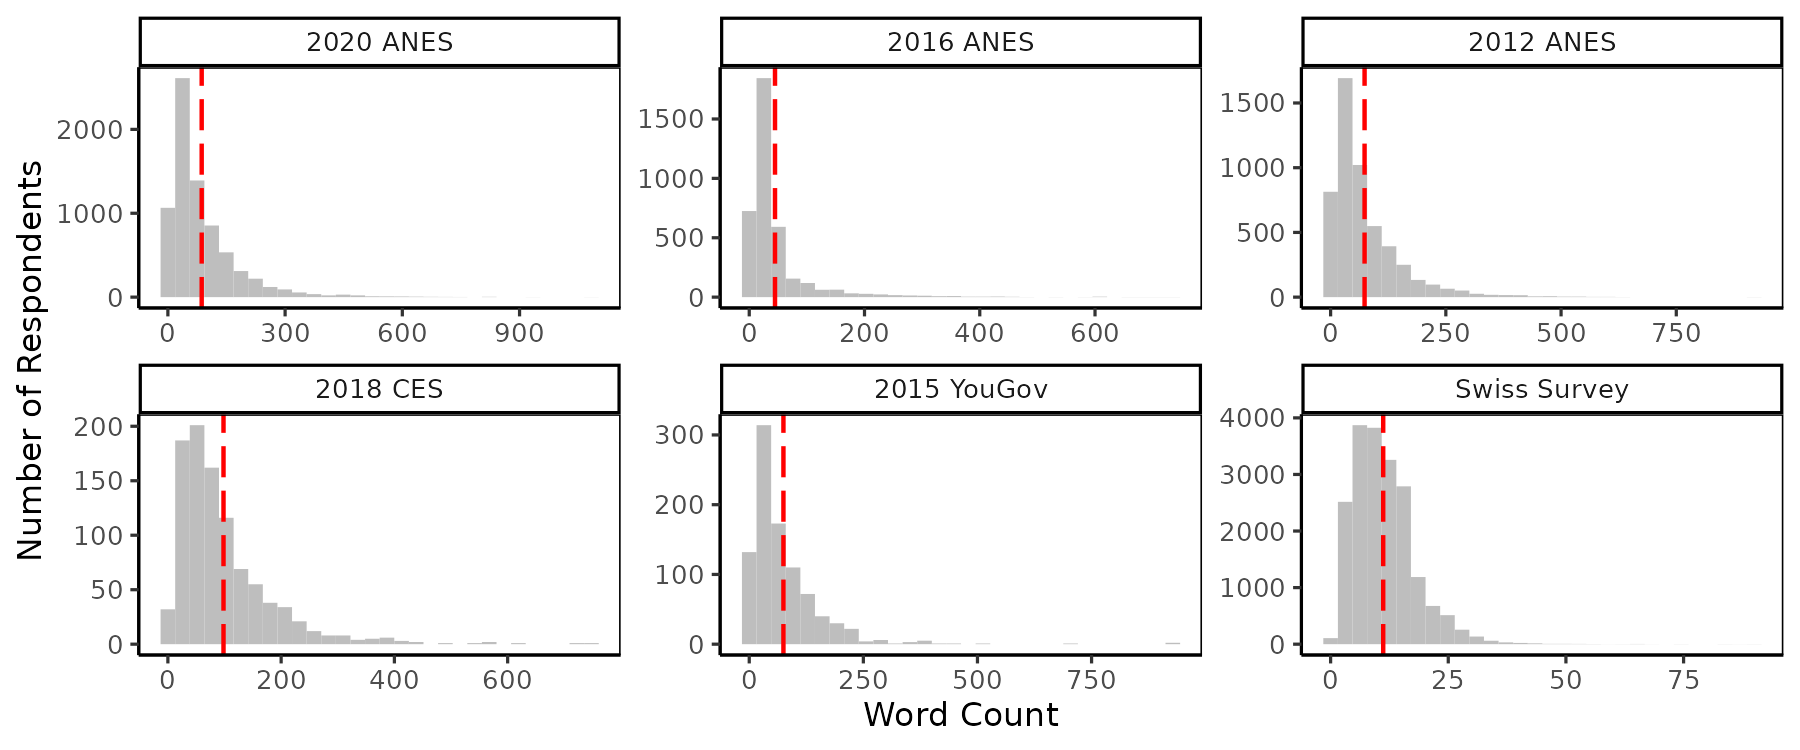
\includegraphics{../fig/wc.png}
	\caption[Total word count across all open-ended responses]{Total word count across all open-ended responses for each survey participant. The dashed red lines indicate the average response lengths in each survey.}\label{fig:wc}
\end{figure}

\begin{figure}[ht]\centering
	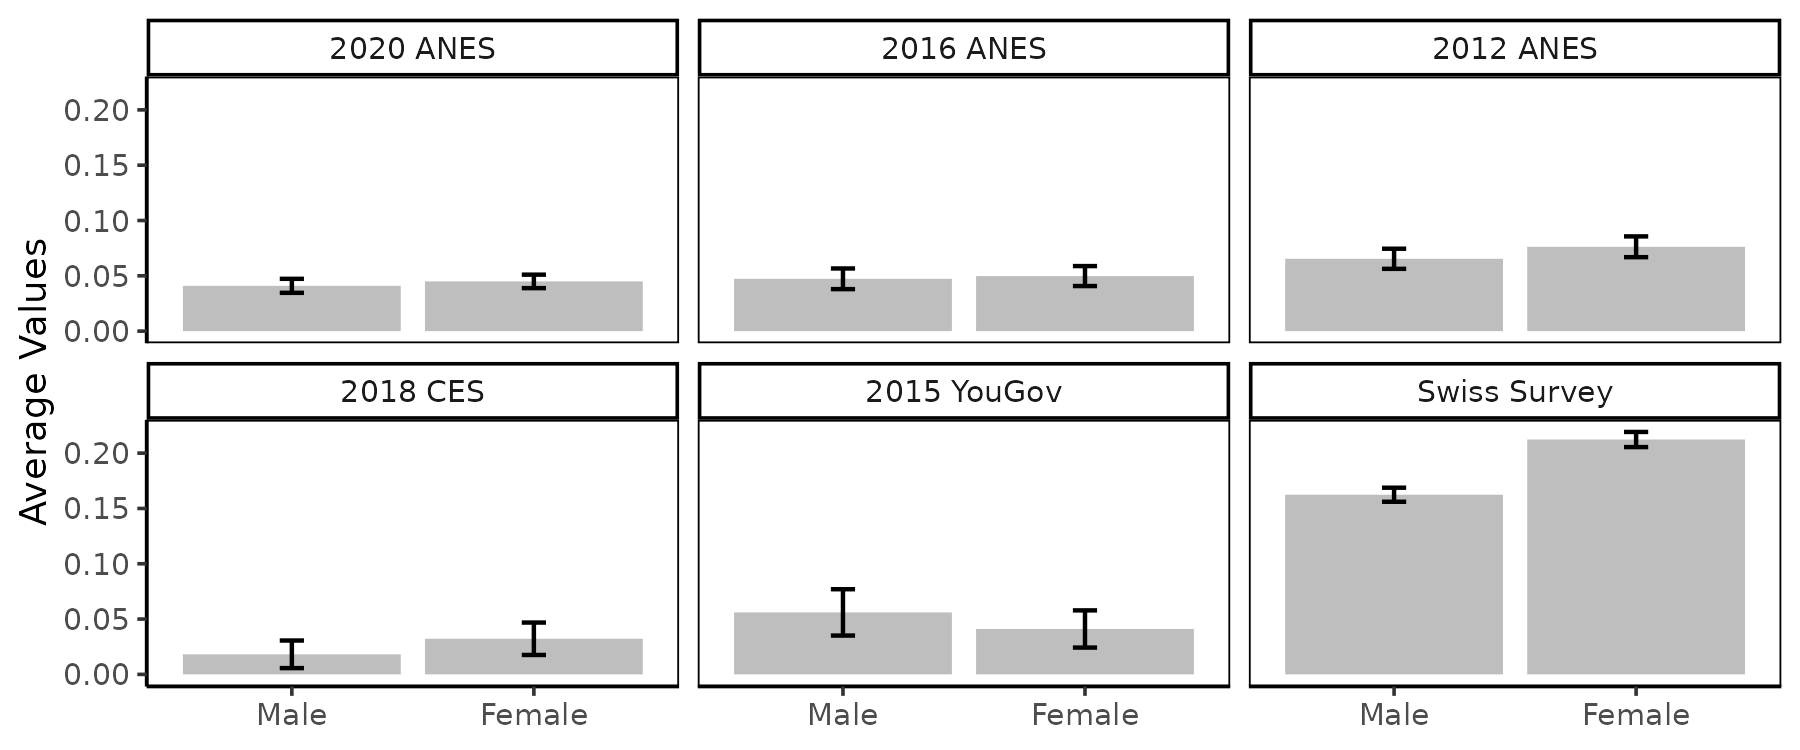
\includegraphics{../fig/noresponse.png}
	\caption{Proportion of non-response comparing male and female survey participants (including 95\% confidence intervals). Gender differences are only significant ($p<.05$) for the Swiss survey. Note, however, that respondents in the Swiss survey were only asked open-ended questions if they voted in the respective referendum.}
\end{figure}


\clearpage
\subsection{Preprocessing and Topic Model Specification}

I rely on the structural topic model framework to extract and differentiate considerations mentioned by respondents. I follow the guidelines in \citet{roberts2014structural} to preprocess our open-ended responses (lowercasing and stemming as well as removing stopwords, punctuation, numbers, and infrequent terms)\footnote{Prior to applying these preprocessing steps, responses are cleaned by removing open-ended item non-response such as `don't know' and correcting spelling errors using an implementation of the Aspell spell-checking algorithm (\url{www.aspell.net}).} and used age, gender, education, party identification, as well as an interaction between education and party identification as covariates for topic prevalence. With the exception of gender, this variable selection is equivalent to the procedure described in \citet{roberts2014structural} for open-ended survey responses such as those included in the ANES. I set the number of topics to 25 in order to focus on the differentiation of broader considerations, but I replicate equivalent results with larger numbers of topics below. Figure~\ref{fig:stm_prop} displays the resulting topic proportions for all data sets included in the analyses along with the most frequent and exclusive (FREX) terms associated with each topic.

\begin{figure}[h]\centering
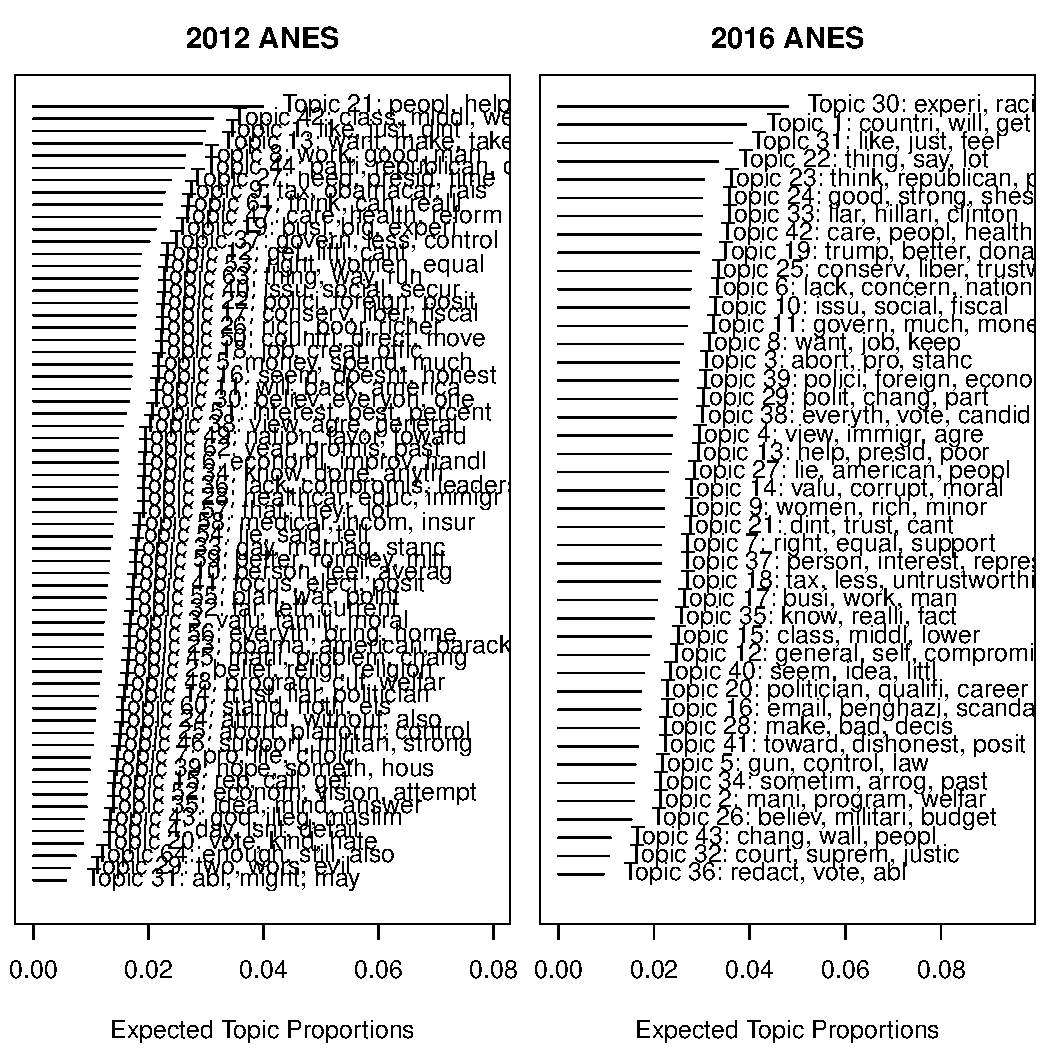
\includegraphics[width=.89\textwidth]{../fig/stm_prop.pdf}
\caption[Estimated topic proportions based on the structural topic model]{Estimated topic proportions based on the structural topic model. See Appendix~\ref{app:robustness}.\ref{app:topicmodel} for details on the model specification.}\label{fig:stm_prop}
\end{figure}


\clearpage
\subsection{Discursive Sophistication Components}\label{app:components}
\begin{figure*}[h]
    \centering
    \begin{subfigure}[h]{0.27\textwidth}
    	\centering
    	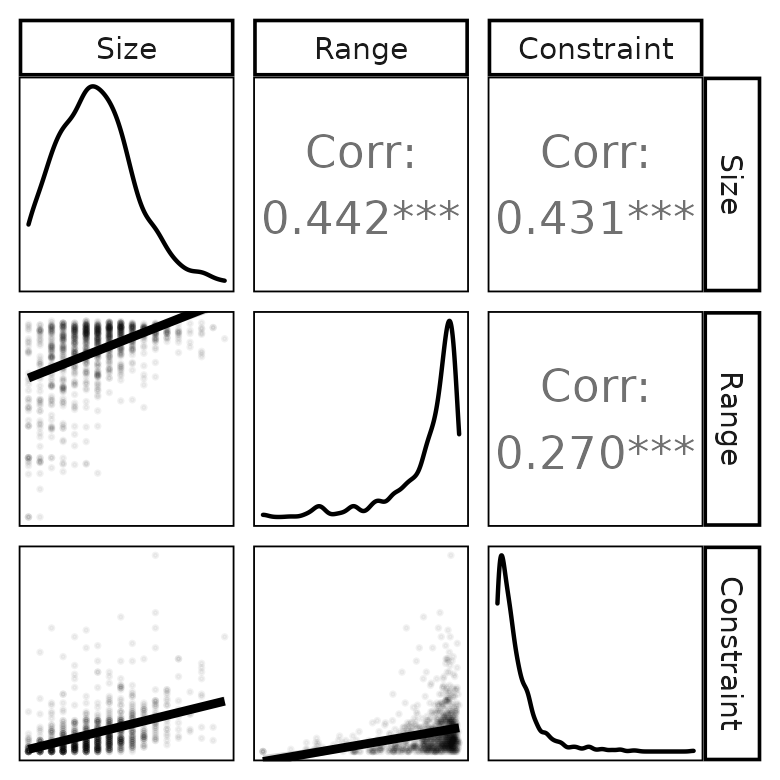
\includegraphics[width=\textwidth]{../fig/cces2018_components.png}
    	\caption{2018 CES}
    \end{subfigure}%
    \begin{subfigure}[h]{0.27\textwidth}
		\centering
		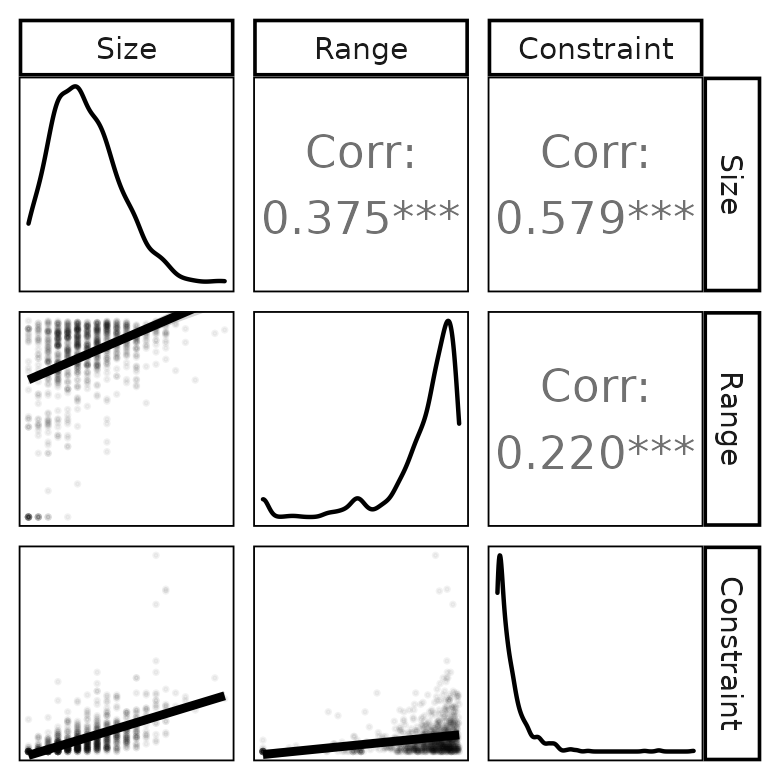
\includegraphics[width=\textwidth]{../fig/yg_components.png}
		\caption{2015 YouGov}
	\end{subfigure}%

    \begin{subfigure}[h]{0.27\textwidth}
    	\centering
    	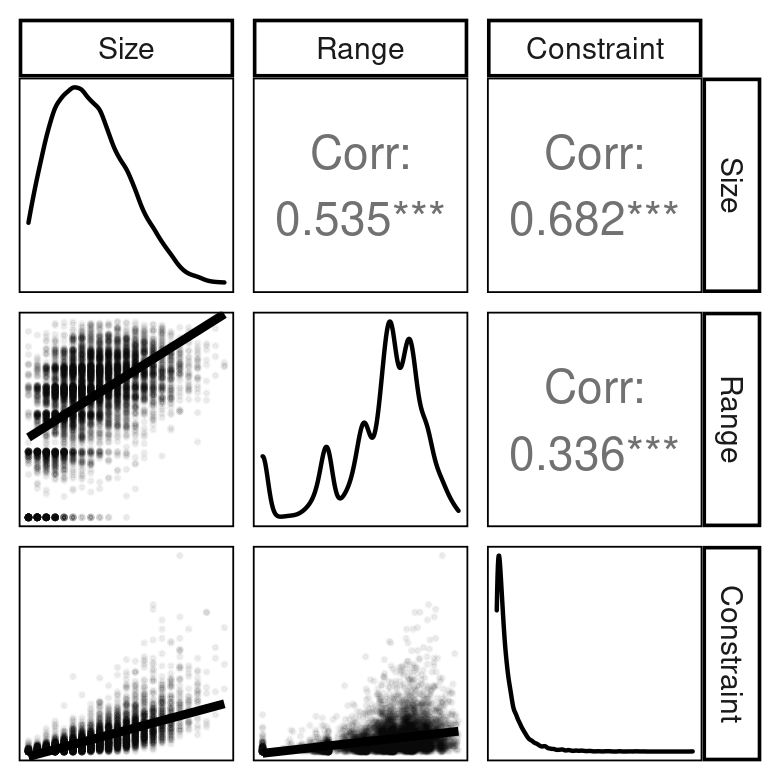
\includegraphics[width=\textwidth]{../fig/anes2020_components.png}
    	\caption{2020 ANES}
    \end{subfigure}%
    \begin{subfigure}[h]{0.27\textwidth}
        \centering
        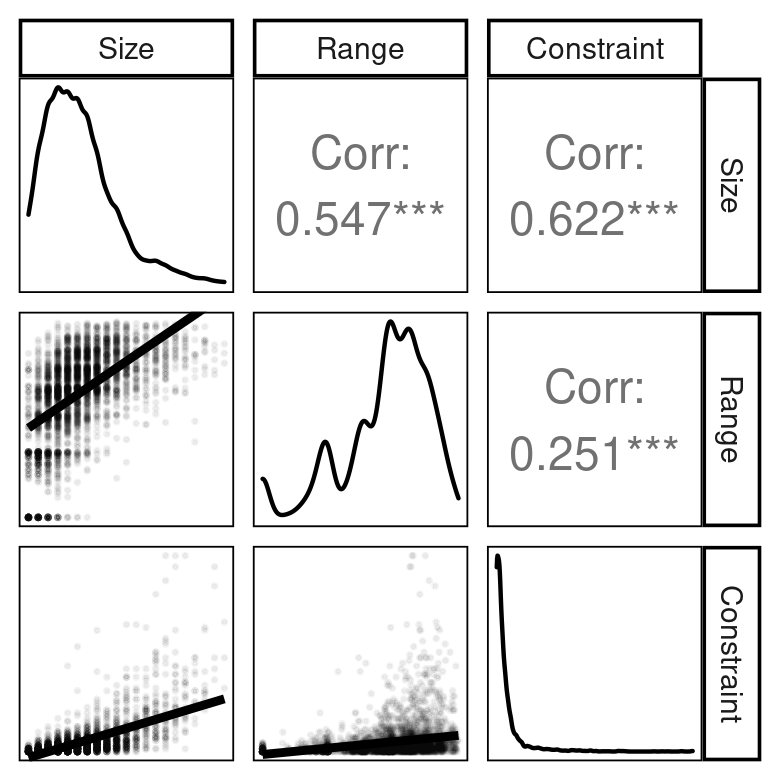
\includegraphics[width=\textwidth]{../fig/anes2016_components.png}
        \caption{2016 ANES}
    \end{subfigure}%
    \begin{subfigure}[h]{0.27\textwidth}
         \centering
         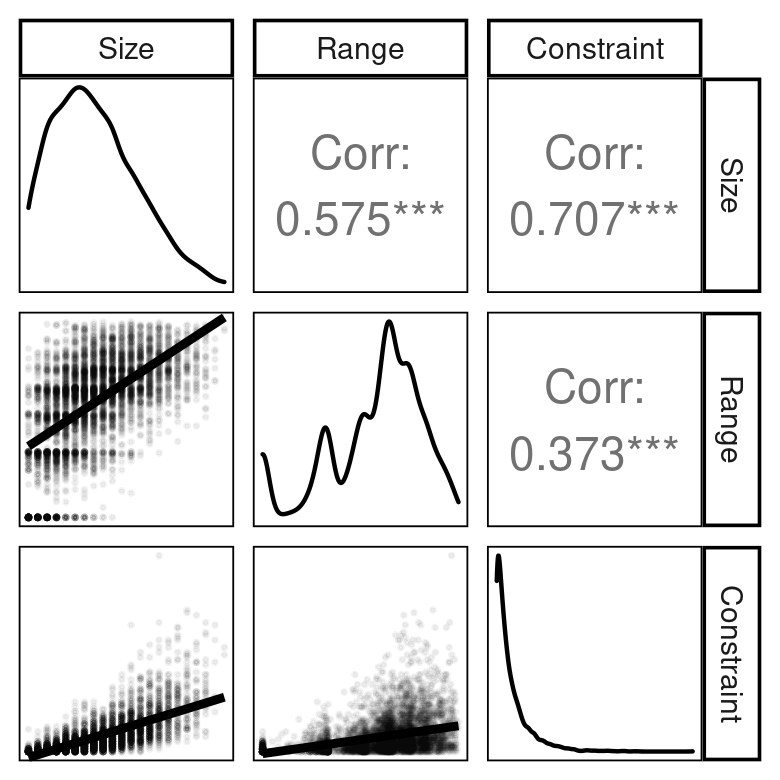
\includegraphics[width=\textwidth]{../fig/anes2012_components.png}
         \caption{2012 ANES}
    \end{subfigure}%

    \begin{subfigure}[h]{0.27\textwidth}
         \centering
         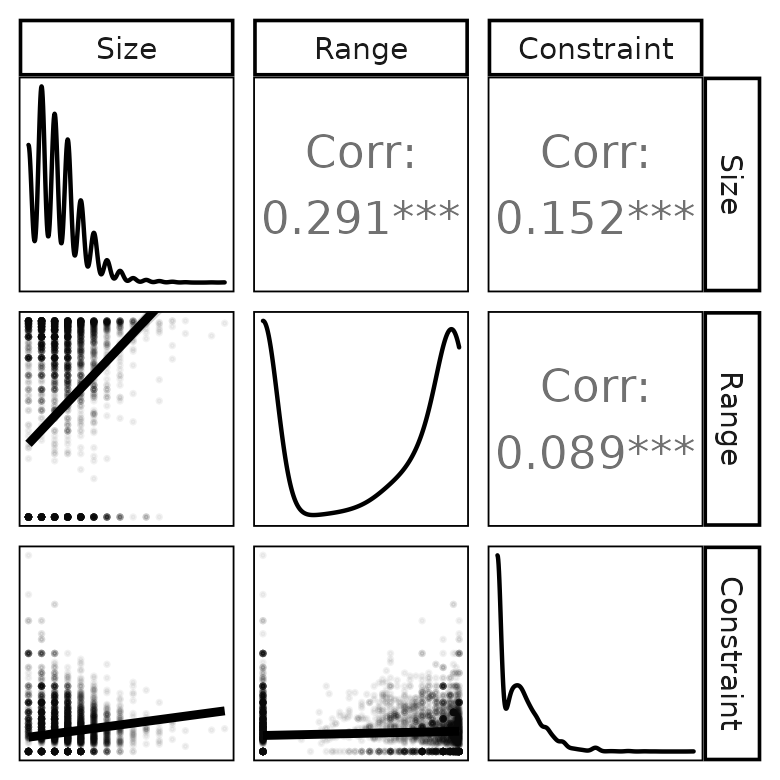
\includegraphics[width=\textwidth]{../fig/french_components.png}
         \caption{Swiss Survey - French}
    \end{subfigure}%
	\begin{subfigure}[h]{0.27\textwidth}
		\centering
		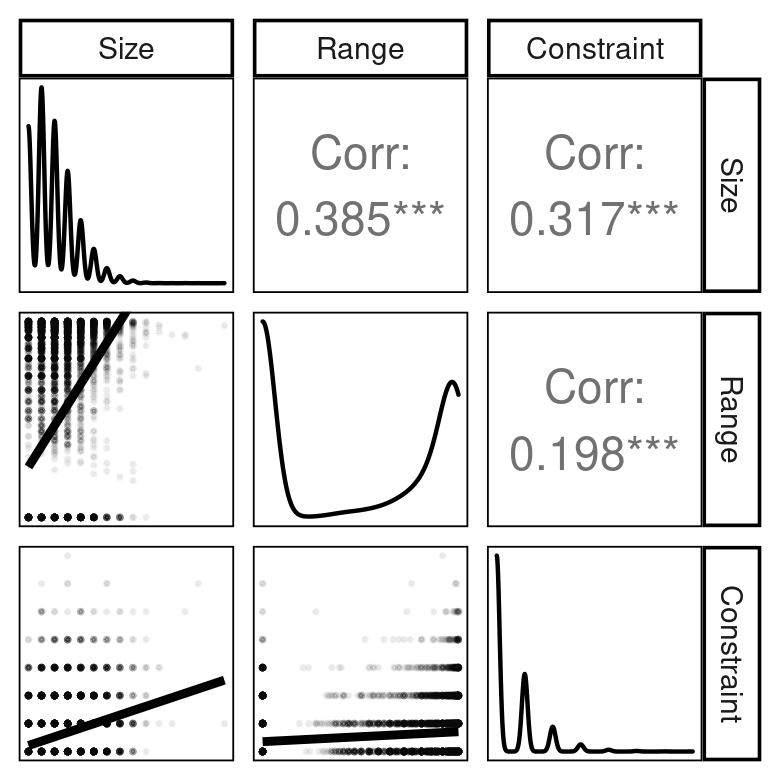
\includegraphics[width=\textwidth]{../fig/german_components.png}
		\caption{Swiss Survey - German}
	\end{subfigure}%
	\begin{subfigure}[h]{0.27\textwidth}
		\centering
		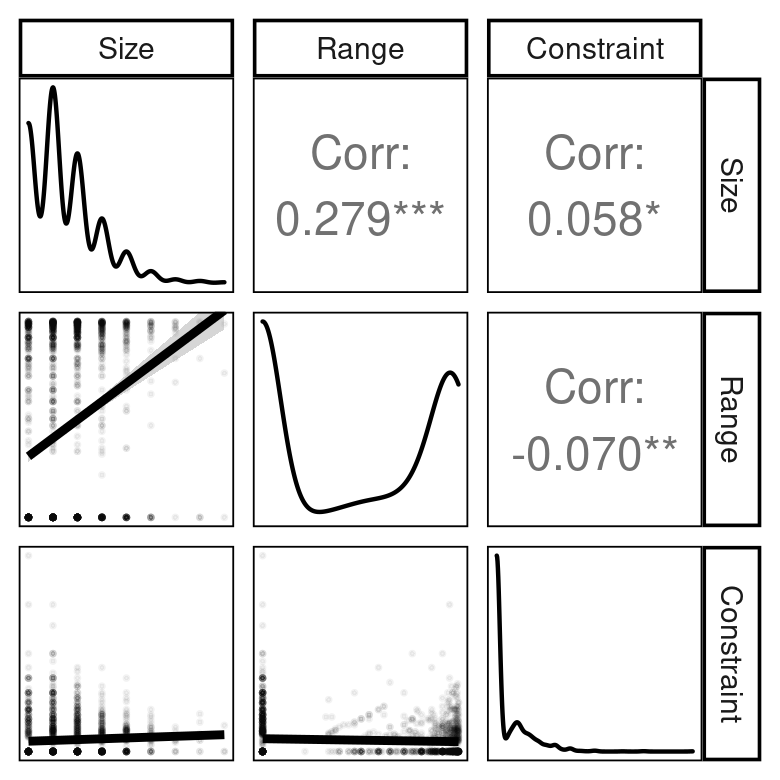
\includegraphics[width=\textwidth]{../fig/italian_components.png}
		\caption{Swiss Survey - Italian}
	\end{subfigure}
    \caption[Correlation matrix of individual components of discursive sophistication.]{Correlation matrix of individual components of discursive sophistication. The plots on the diagonal display univariate densities for each component. The panels in the lower triangular display the scatter plot of two measures as well as a linear fit. %The upper triangular displays the correlation coefficient.
     }\label{fig:components}
\end{figure*}



\clearpage
\section{Robustness Checks}\label{app:robustness}

\subsection{PreText Analysis}\label{app:topicmodel}

The first component of discursive sophistication (\textit{size}) relies on quantities extracted from structural topic models \citep{roberts2014structural}. As with any other text-as-data approach, a necessary first step before estimating the topic model is to preprocess the raw text and convert it into a document term matrix \citep[DTM, see for example][]{manning2008introduction}. Common preprocessing procedures include stemming and lowercasing, as well as the removal of numbers, punctuation, stopwords, and infrequent terms. However, topic models and other unsupervised learning techniques can be sensitive to these preprocessing choices. To address this issue, \citet{denny2018text} recommend that researchers compare DTMs under all possible preprocessing regimes. The authors propose \textit{preText scores} as a measure to quantify the extent to which varying preprocessing regimes may yield unusual results compared to a baseline without any preprocessing. Following the procedure outlined in \citet{denny2018text}, Figure~\ref{fig:pretext} displays the results of a linear model regressing preText scores resulting from all possible preprocessing regimes on each individual step for a random subset of 500 open-ended responses in each of the surveys included in the analyses. Significant coefficients indicate that the topic model results may be sensitive to the respective preprocessing step.

\begin{figure}[h]
\centering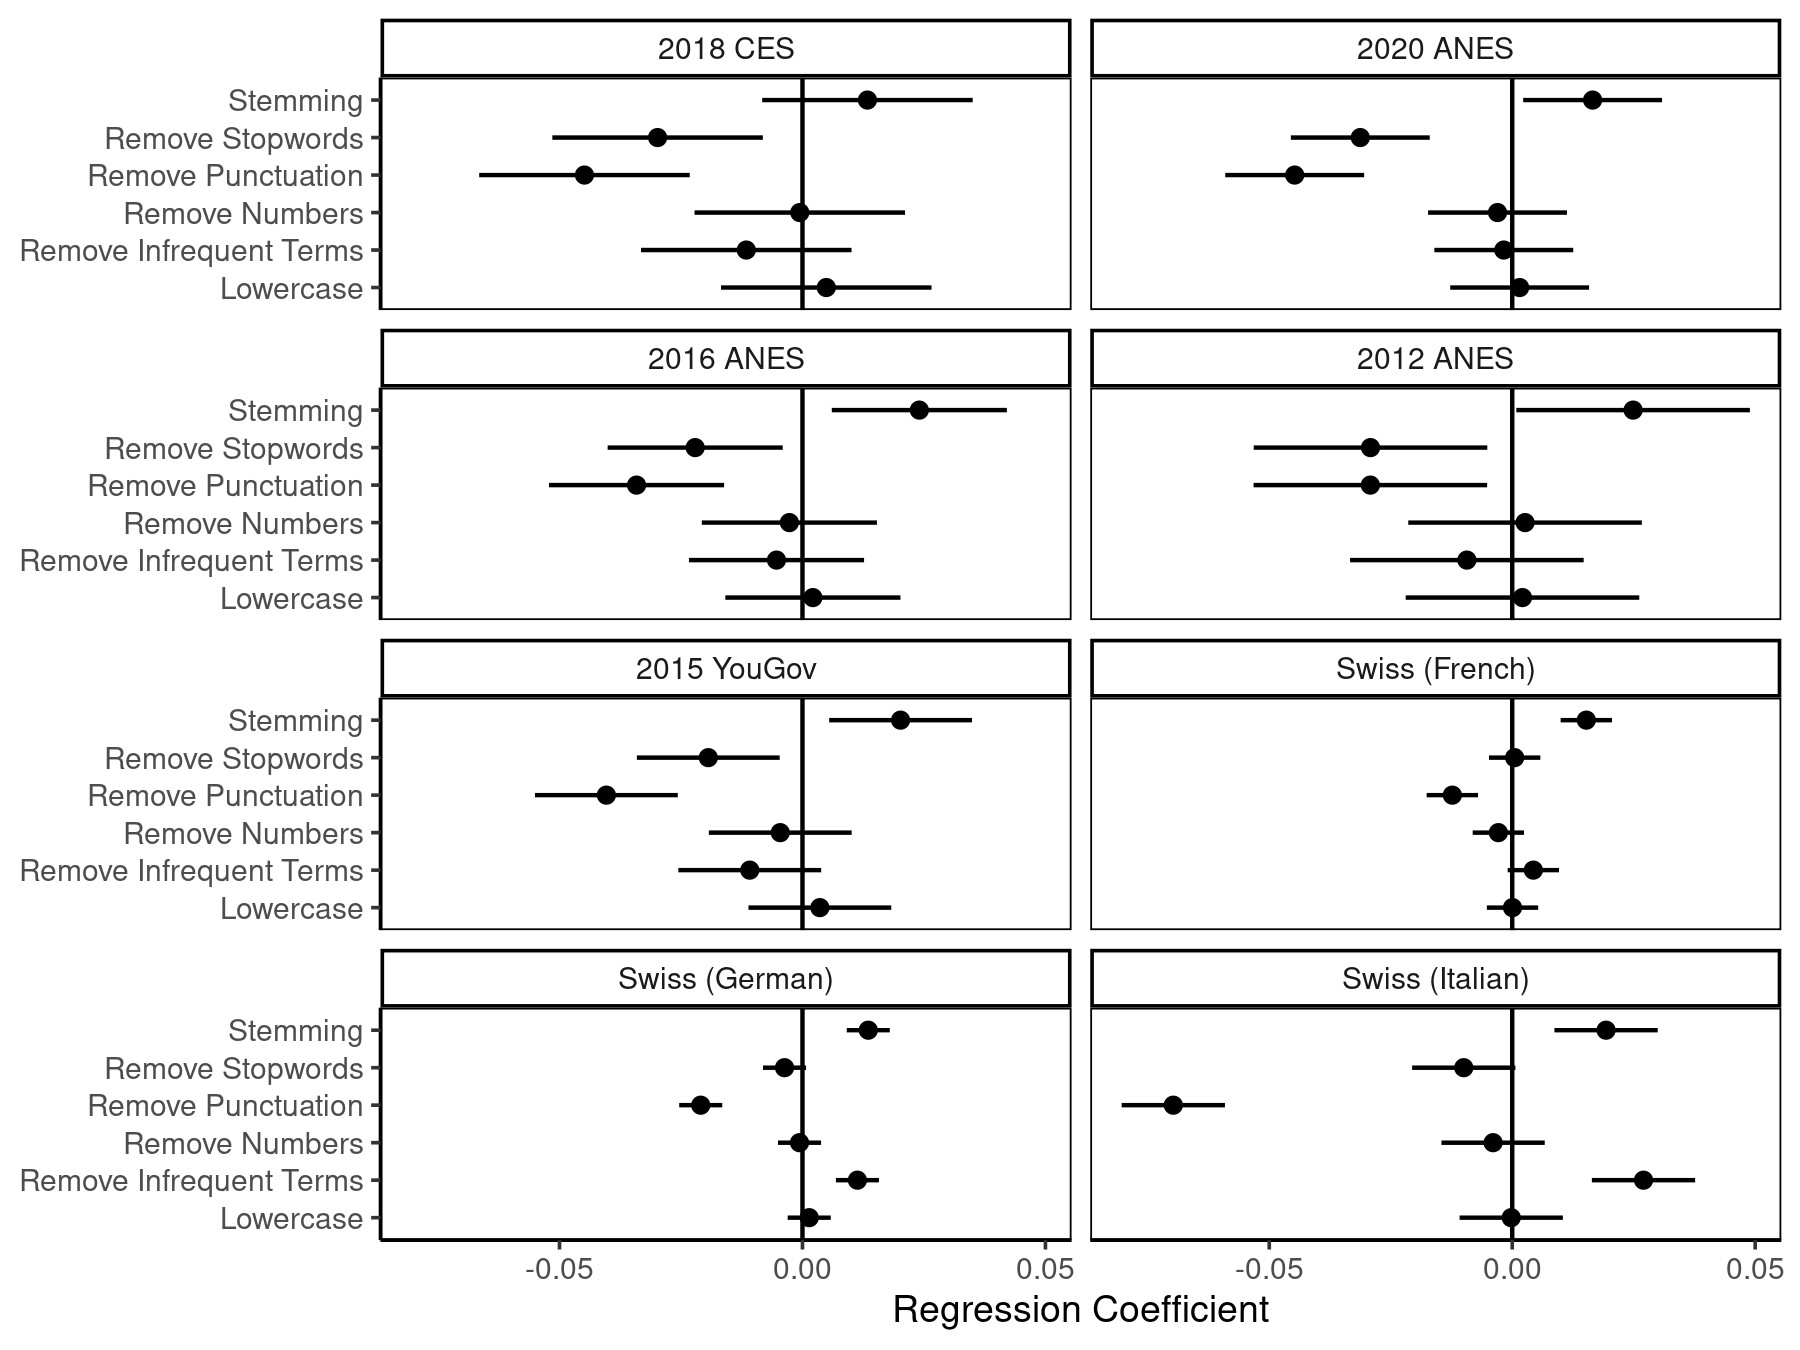
\includegraphics[scale=.9]{../fig/pretext.png}
    \caption[PreText analysis of preprocessing decisions of open-ended responses across all datasets]{PreText analysis of preprocessing decisions of open-ended responses across all datasets. Regression coefficients display the effects of each of the six preprocessing choices on the resulting preText score.}\label{fig:pretext}
\end{figure}


\clearpage
\subsection{Discursive Sophistication for Varying Model Specifications}

According to the analysis in Figure~\ref{fig:pretext}, our results may be particularly sensitive to stemming and the removal of stopwords or punctuation. \citet{denny2018text}, however, emphasize that the most important consideration in choosing preprocessing steps are theoretical. Given that the purpose of our topic model is to extract considerations related to political preferences, there are no theoretical reasons to incorporate punctuation since it does not contain any relevant content. It is less obvious from a theoretical perspective whether to use stemming or to remove stopwords from our open-ended responses, although it might be preferable in order to increase computational efficiency. Following \citet{denny2018text}, I proceed by assessing to what extent discursive sophistication varies across the alternative preprocessing regimes identified as potentially influential. In addition, I consider another crucial modeling choice when working with topic models: determining the total number of topics $k$ to be estimated.

Figure~\ref{fig:pretext_robustness} examines whether the proposed measure of discursive sophistication is sensitive to changing the number of topics $k$, stemming, and the removal of stopwords. The y-axis depicts the preferred preprocessing regime including all steps discussed above while the x-axis plots discursive sophistication resulting from alternative specifications. The panels on the left compare the preferred specification to discursive sophistication based on a larger number of topics ($k=35$). The center panels does not use stemming as part of the preprocessing. The panels on the right do not remove stopwords prior to estimating the topic model. Across all data sets, discursive sophistication scores are highly correlated and therefore insensitive to preprocessing choices. Thus, the substantive results discussed in the main text are robust for alternative preprocessing regimes or varying numbers of topics.


\begin{figure}[h]\centering
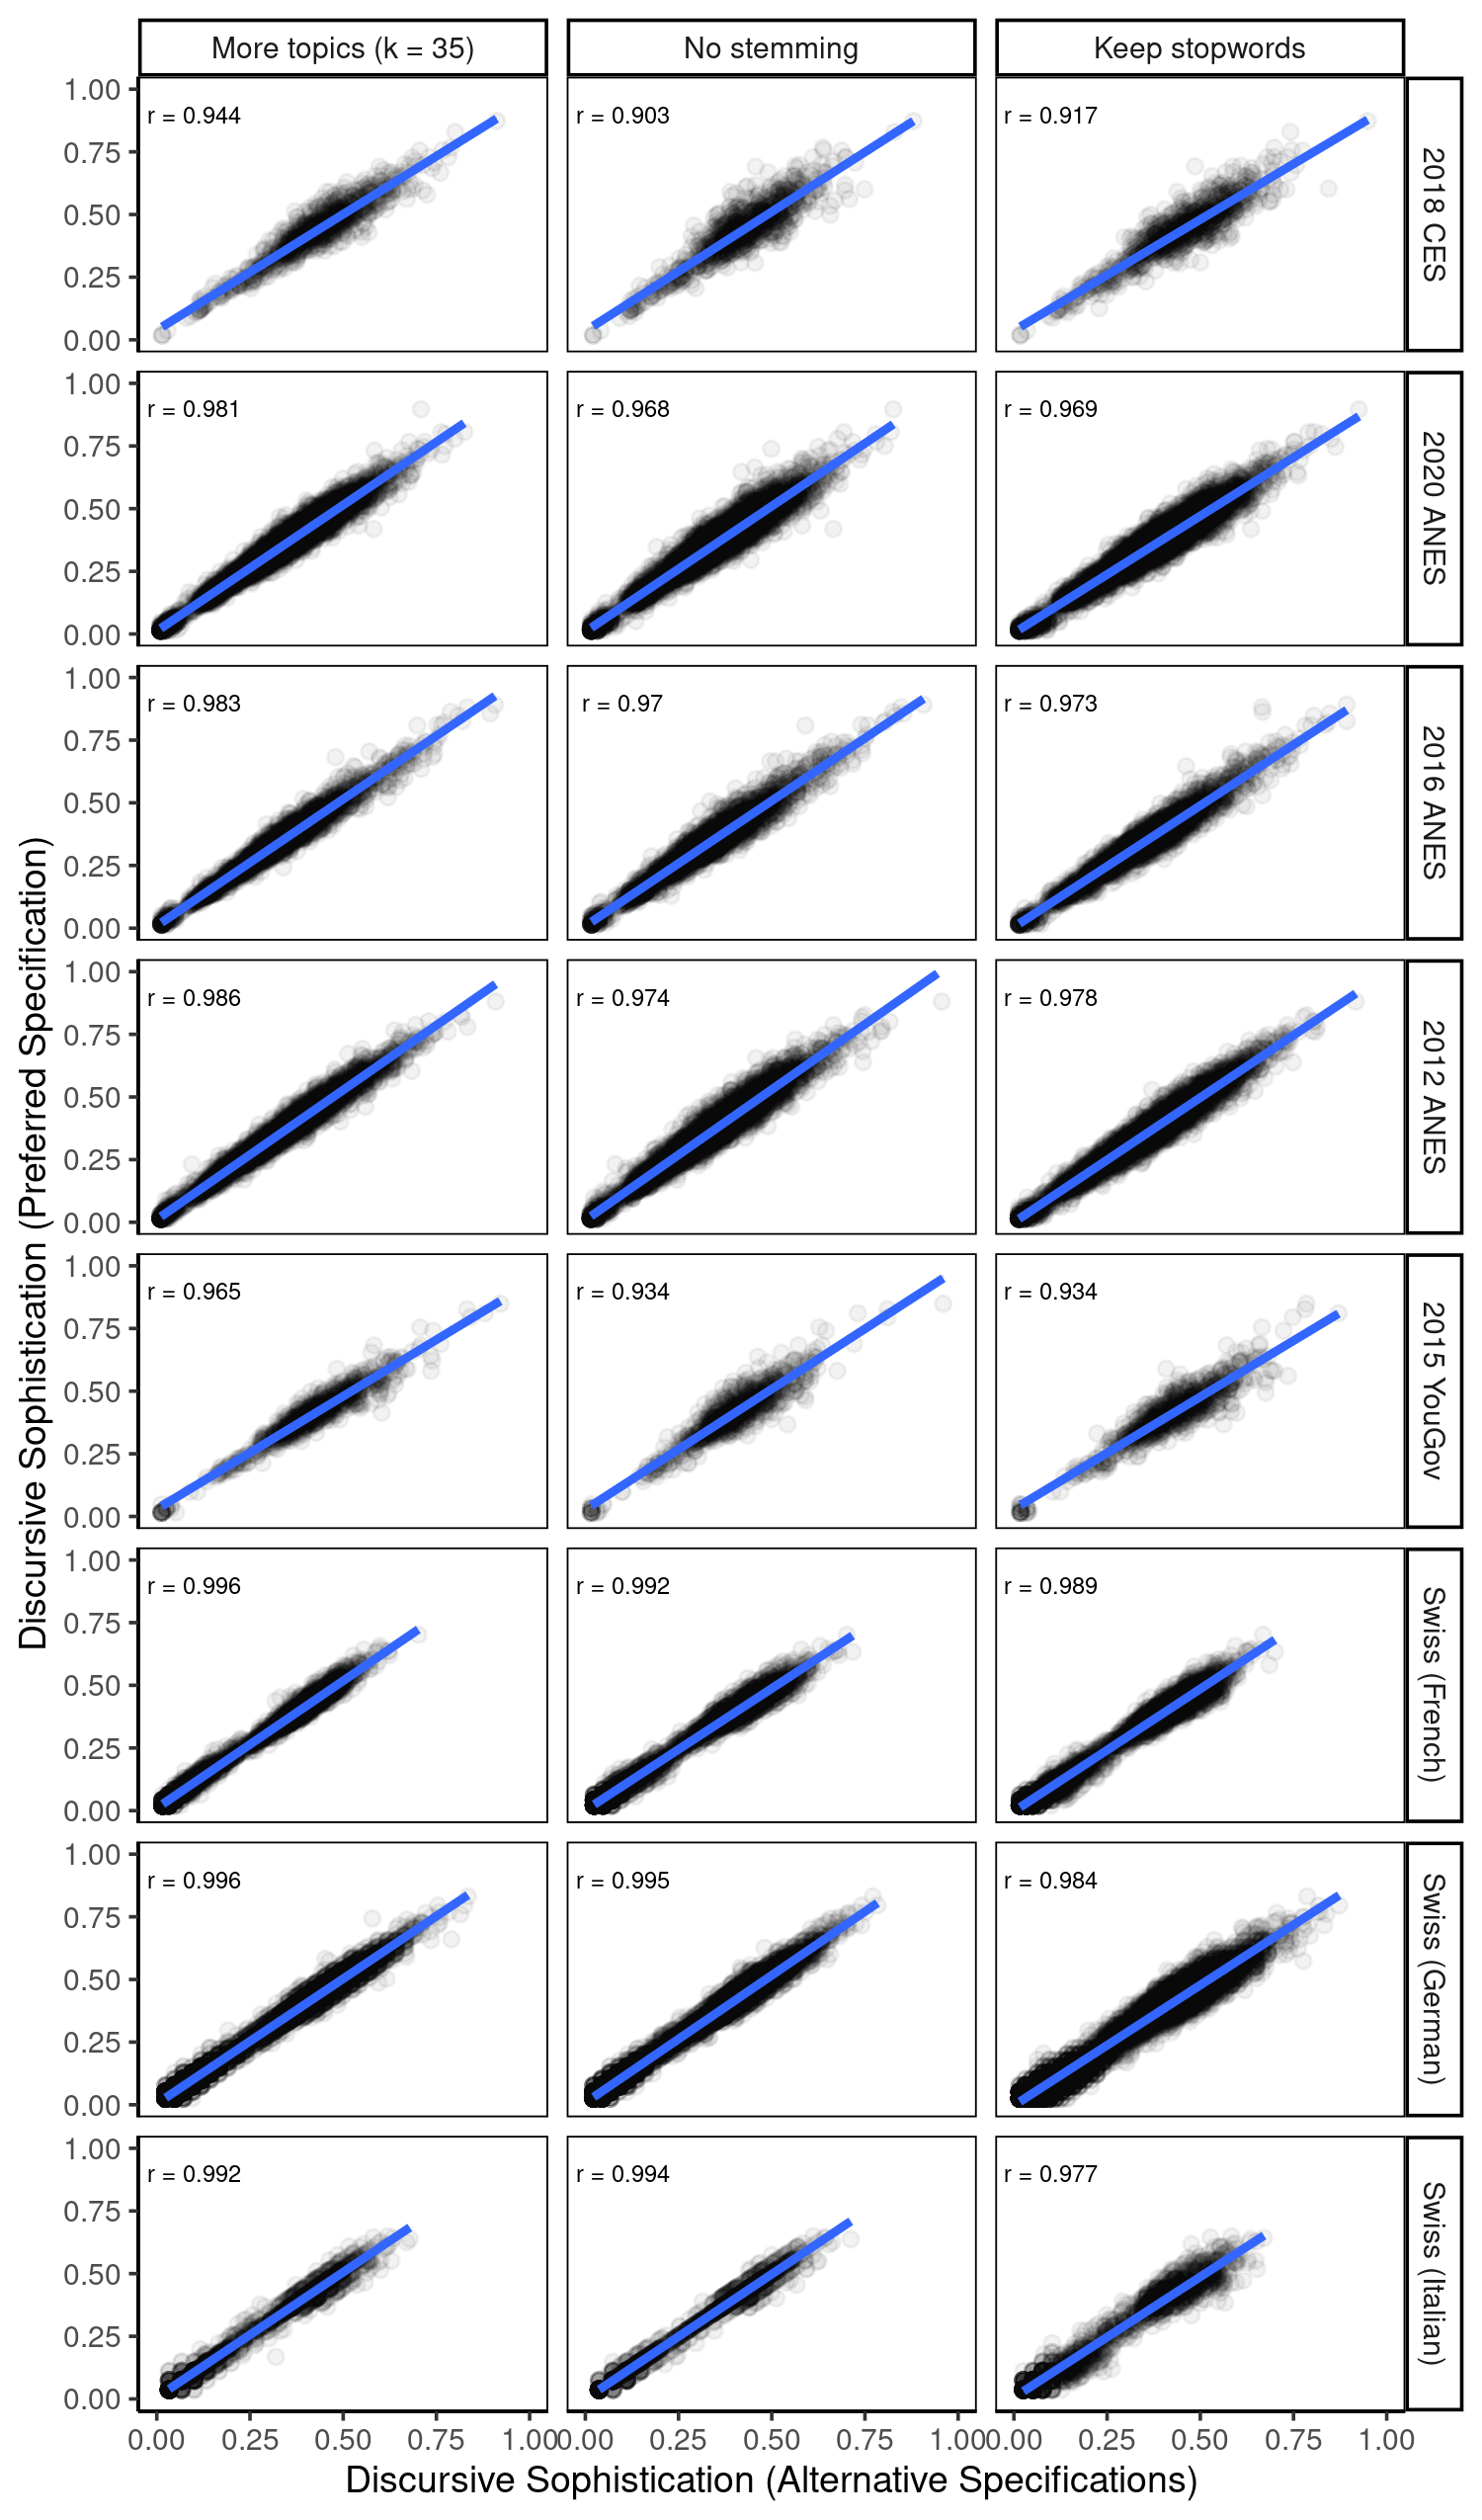
\includegraphics{/data/Dropbox/Uni/projects/2016/knowledge/fig/pretext_robustness.png}
\caption[Robustness of discursive sophistication measure for different preprocessing choices and topic model specifications]{Robustness of discursive sophistication measure for different preprocessing choices and topic model specifications.}\label{fig:pretext_robustness}
\end{figure}

\clearpage
\subsection{Controlling for Personality and Verbal Skills}\label{app:personality}

\begin{figure}[h]\centering
	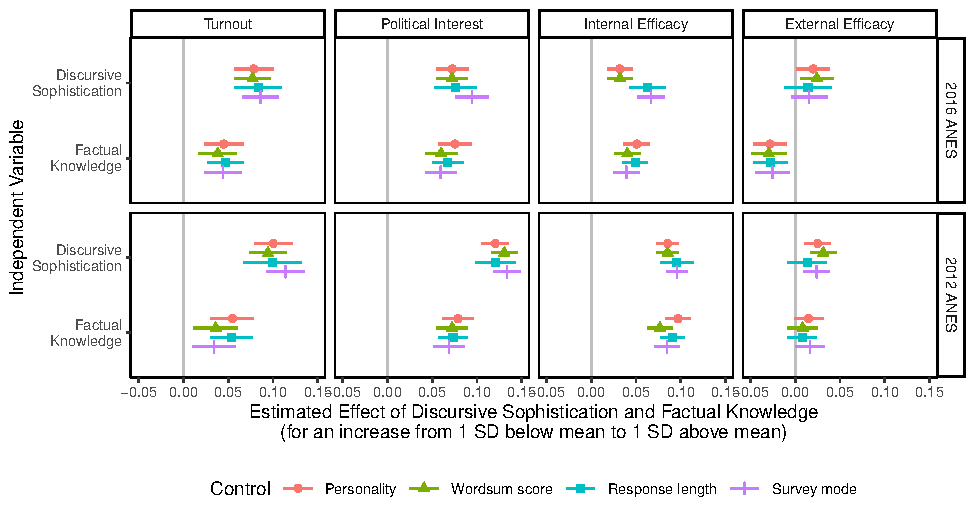
\includegraphics{../fig/knoweff_robust.pdf}
	\caption{Effects of sophistication on internal efficacy, external efficacy, non-conventional participation, and turnout in the 2012 and 2016 ANES. For each dependent variable, the figure displays the average marginal effects (AME) for each sophistication measure (including 95\% confidence intervals). Model estimates are based on logistic regression (turnout) or OLS (political interest, internal efficacy, external efficacy). Compared to the specification used in Figure~2 in the main text (controlling for gender, education, income, age, race, and church attendance), the models displayed here include additional controls for personality (extraversion, openness to experience, being reserved), survey mode (online vs. face-to-face), verbal skills (Wordsum score), and overall verbosity (response length).}\label{fig:knoweff_robust}
\end{figure}

%\vspace{1em}

\paragraph{Description of additional control variables:}

\begin{itemize}
	\item \textit{Personality}: Components of the Ten Item Personality Inventory (TIPI) measuring the ``Big Five'' personality traits measuring extraversion, openness to experience, being reserved.
	\item \textit{Survey Mode}: Dichotomous indicator for face-to-face vs. online samples of the ANES surveys.
	\item \textit{Wordsum vocabulary scores}: Modified version of the GSS wordsum vocabulary test consisting of 10 terms.
	\item \textit{Response length}: Total number of words in the collection of open-ended responses by each individual.
\end{itemize}

\clearpage
\subsection{Discursive Sophistication and Uncertainty in Ideological Placements}\label{app:placement}

\begin{figure}[h]\centering
	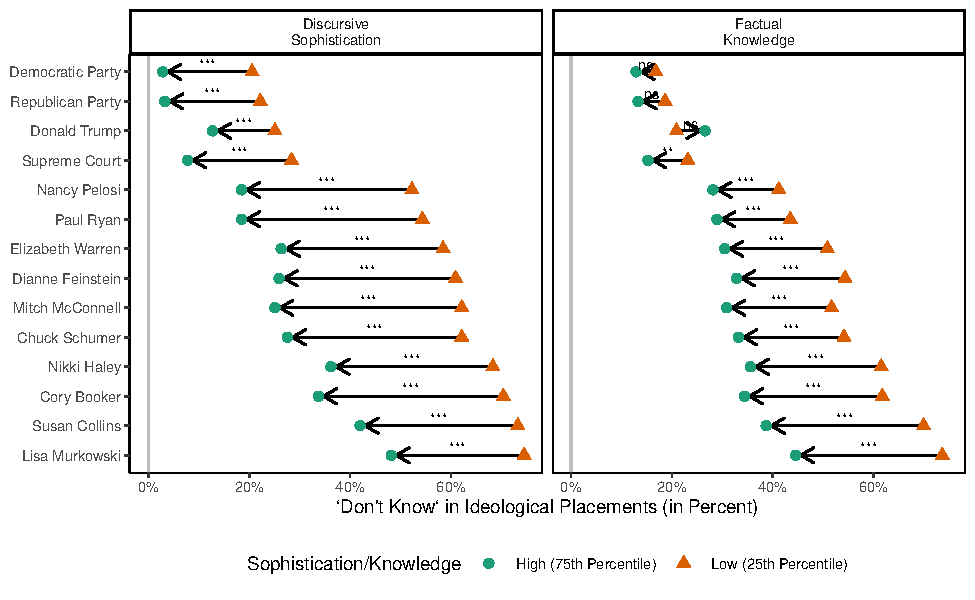
\includegraphics{../fig/placements_dk.pdf}
	\caption{Effects of sophistication on the probability of respondents to answer `Don't Know' when asked to place individual politicians, parties, and institutions on the ideological spectrum from liberal to conservative in the 2018 CES. The figure shows the expected change comparing low (25th percentile) and high (75th percentile) levels of discursive sophistication / factual knowledge. Differences are statistically significant at: $^{*}$p$<$0.05; $^{**}$p$<$0.01; $^{***}$p$<$0.001.}\label{fig:placements_dk}
\end{figure}

\begin{figure}[h]\centering
	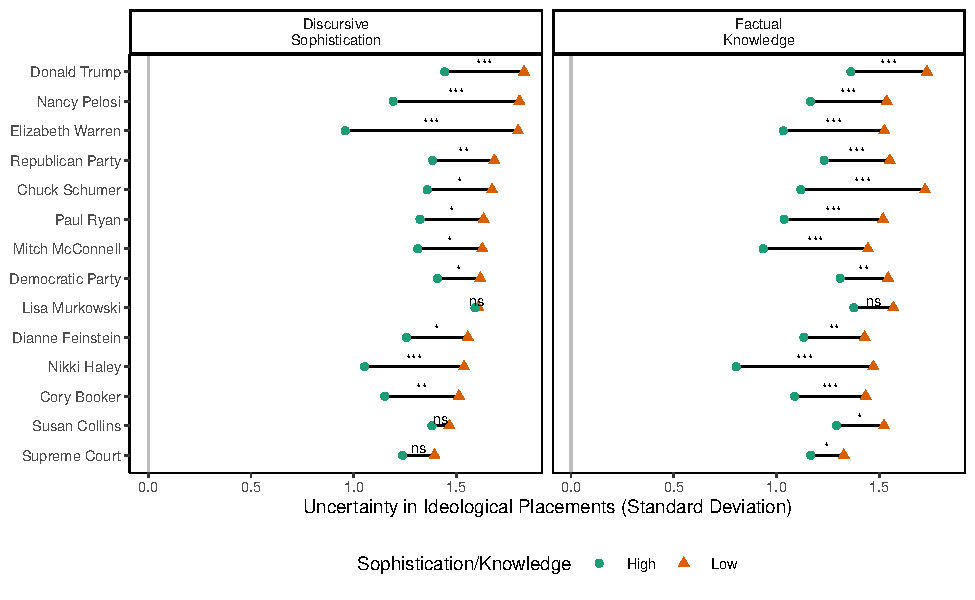
\includegraphics{../fig/placements.pdf}
	\caption{Effects of sophistication on the uncertainty around ideological placements of  politicians, parties, and institutions in the 2018 CES (measured in standard deviations). The figure shows the expected change comparing low (25th percentile) and high (75th percentile) levels of discursive sophistication / factual knowledge. Differences are statistically significant at: $^{*}$p$<$0.05; $^{**}$p$<$0.01; $^{***}$p$<$0.001.}\label{fig:placements}
\end{figure}

\clearpage
\subsection{Discursive Sophistication and Ideological Proximity Voting}\label{app:proximity}

\begin{figure}[h]\centering
	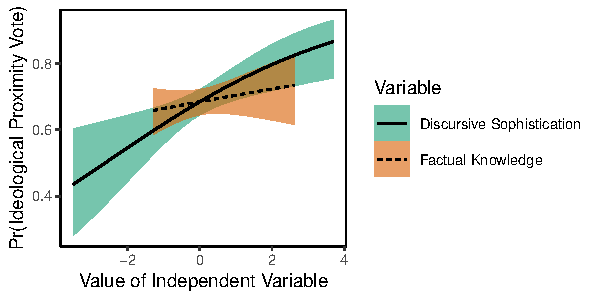
\includegraphics{../fig/correct_vote.pdf}
	\caption{Expected probability to vote for the senatorial candidate based on ideological proximity as a function of political sophistication (including 95\% confidence intervals). Estimates are based on a logistic regression including controls for sociodemographic variables. The predictions are made by setting covariates equal to their mean (continuous) or median (categorical) value. Full regression results are displayed in Table~\ref{tab:correct_vote}.}\label{fig:correct_vote}
\end{figure}


% Table created by stargazer v.5.2.3 by Marek Hlavac, Social Policy Institute. E-mail: marek.hlavac at gmail.com
% Date and time: Mon, Aug 15, 2022 - 10:29:53 PM
% Requires LaTeX packages: dcolumn 
\begin{table}[!htbp] \centering 
  \caption{Logistic regression predicting ideological proximity-based voting for
          US Senators in the 2018 CES. Standard errors in parentheses. 
          Estimates are used for Figure \ref{fig:correct_vote}.} 
  \label{tab:correct_vote} 
\footnotesize 
\begin{tabular}{@{\extracolsep{-25pt}}lD{.}{.}{-3} } 
\\[-1.8ex]\hline 
\hline \\[-1.8ex] 
 & \multicolumn{1}{c}{\textit{Dependent variable:}} \\ 
\cline{2-2} 
 & \multicolumn{1}{c}{Ideological Proximity Vote} \\ 
\hline \\[-1.8ex] 
 Discursive Soph. & 0.296^{**} \\ 
  & (0.097) \\ 
  Factual Knowledge & 0.093 \\ 
  & (0.101) \\ 
  Female & -0.226 \\ 
  & (0.188) \\ 
  Age & 0.016^{**} \\ 
  & (0.005) \\ 
  Black & -0.177 \\ 
  & (0.328) \\ 
  College Degree & 0.408^{*} \\ 
  & (0.200) \\ 
  Household Income & 0.322 \\ 
  & (0.441) \\ 
  Church Attendance & 0.104 \\ 
  & (0.274) \\ 
  Constant & -0.209 \\ 
  & (0.344) \\ 
 \hline \\[-1.8ex] 
Observations & \multicolumn{1}{c}{611} \\ 
Akaike Inf. Crit. & \multicolumn{1}{c}{746.658} \\ 
\hline 
\hline \\[-1.8ex] 
\textit{Note:}  & \multicolumn{1}{r}{$^{*}$p$<$0.05; $^{**}$p$<$0.01; $^{***}$p$<$0.001} \\ 
\end{tabular} 
\end{table} 


\clearpage
\subsection{Discursive Sophistication and Trust in Different News Sources}\label{app:media}

\begin{figure}[h]\centering
	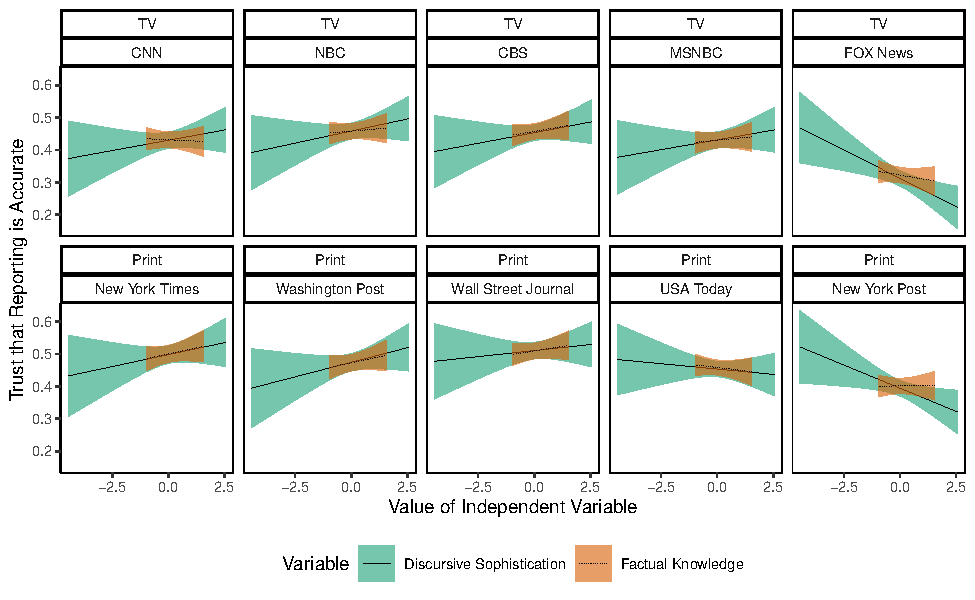
\includegraphics{../fig/media_trust.pdf}
	\caption{Bivariate linear associations between trust in different news outlets and political sophistication in the 2019 MTurk Study (including 95\% confidence intervals).}\label{fig:media_trust}
\end{figure}
% Average trust in news media as a function of political sophistication in the 2019 MTurk Study (including 95\% confidence intervals). Estimates are based on bivariate linear regressions.

\clearpage
\subsection{Personality and Verbal Skills as Predictors of Discursive Sophistication}\label{app:determinants_rob}


% Table created by stargazer v.5.2.3 by Marek Hlavac, Social Policy Institute. E-mail: marek.hlavac at gmail.com
% Date and time: Mon, Feb 27, 2023 - 07:48:58 PM
% Requires LaTeX packages: dcolumn 
\begin{table}[!htbp] \centering 
  \caption{Personality, verbal skills, and survey mode as predictors
          of discursive sophistication in the 2016 and 2012 ANES.} 
  \label{tab:determinants_rob_disc} 
\footnotesize 
\begin{tabular}{@{\extracolsep{-5pt}}lD{.}{.}{-3} D{.}{.}{-3} D{.}{.}{-3} D{.}{.}{-3} } 
\\[-1.8ex]\hline 
\hline \\[-1.8ex] 
 & \multicolumn{4}{c}{\textit{Dependent variable:}} \\ 
\cline{2-5} 
\\[-1.8ex] & \multicolumn{4}{c}{Discursive Sophistication} \\ 
 & \multicolumn{2}{c}{2016 ANES} & \multicolumn{2}{c}{2012 ANES} \\ 
\\[-1.8ex] & \multicolumn{1}{c}{(1)} & \multicolumn{1}{c}{(2)} & \multicolumn{1}{c}{(3)} & \multicolumn{1}{c}{(4)}\\ 
\hline \\[-1.8ex] 
 Personality: Extraversion & 0.042 & 0.046 & -0.078 & -0.071 \\ 
  & (0.069) & (0.069) & (0.061) & (0.060) \\ 
  Personality: Openness to Experience & 0.228^{**} & 0.224^{**} & 0.259^{***} & 0.277^{***} \\ 
  & (0.079) & (0.079) & (0.064) & (0.064) \\ 
  Personality: Reserved & -0.114^{*} & -0.112 & -0.125^{*} & -0.128^{*} \\ 
  & (0.058) & (0.058) & (0.050) & (0.050) \\ 
  Verbal Skills (Wordsum score) & 0.945^{***} & 0.880^{***} & 1.120^{***} & 0.915^{***} \\ 
  & (0.084) & (0.086) & (0.070) & (0.072) \\ 
  Survey Mode (Online) & -0.900^{***} & -0.913^{***} & -0.425^{***} & -0.460^{***} \\ 
  & (0.035) & (0.035) & (0.031) & (0.031) \\ 
  Factual Knowledge &  & 0.059^{***} &  & 0.176^{***} \\ 
  &  & (0.017) &  & (0.017) \\ 
  Female & -0.061 & -0.052 & -0.029 & 0.013 \\ 
  & (0.032) & (0.032) & (0.027) & (0.027) \\ 
  Age & 0.0003 & -0.00005 & 0.005^{***} & 0.003^{***} \\ 
  & (0.001) & (0.001) & (0.001) & (0.001) \\ 
  Black & -0.070 & -0.075 & 0.096^{*} & 0.125^{**} \\ 
  & (0.059) & (0.059) & (0.039) & (0.039) \\ 
  PID: Democrat & 0.039 & 0.033 & 0.056 & 0.061 \\ 
  & (0.039) & (0.039) & (0.032) & (0.032) \\ 
  PID: Republican & 0.067 & 0.068 & 0.036 & 0.026 \\ 
  & (0.041) & (0.041) & (0.036) & (0.036) \\ 
  Education: High School & 0.120 & 0.114 & 0.118^{*} & 0.081 \\ 
  & (0.079) & (0.079) & (0.054) & (0.054) \\ 
  Education: Some College & 0.339^{***} & 0.334^{***} & 0.325^{***} & 0.266^{***} \\ 
  & (0.076) & (0.076) & (0.054) & (0.053) \\ 
  Education: Bachelor's Degree & 0.549^{***} & 0.538^{***} & 0.514^{***} & 0.426^{***} \\ 
  & (0.081) & (0.081) & (0.060) & (0.060) \\ 
  Education: Graduate Degree & 0.584^{***} & 0.571^{***} & 0.604^{***} & 0.501^{***} \\ 
  & (0.085) & (0.085) & (0.066) & (0.066) \\ 
  Household Income & 0.199^{***} & 0.187^{**} & 0.214^{***} & 0.151^{**} \\ 
  & (0.060) & (0.060) & (0.050) & (0.050) \\ 
  Church Attendance & 0.006 & 0.003 & 0.079^{*} & 0.079^{*} \\ 
  & (0.048) & (0.048) & (0.039) & (0.039) \\ 
  Constant & -0.651^{***} & -0.569^{***} & -1.259^{***} & -0.986^{***} \\ 
  & (0.121) & (0.123) & (0.095) & (0.097) \\ 
 \hline \\[-1.8ex] 
Observations & \multicolumn{1}{c}{3,018} & \multicolumn{1}{c}{3,014} & \multicolumn{1}{c}{4,696} & \multicolumn{1}{c}{4,696} \\ 
R$^{2}$ & \multicolumn{1}{c}{0.267} & \multicolumn{1}{c}{0.270} & \multicolumn{1}{c}{0.180} & \multicolumn{1}{c}{0.199} \\ 
\hline 
\hline \\[-1.8ex] 
\textit{Note:}  & \multicolumn{4}{r}{$^{*}$p$<$0.05; $^{**}$p$<$0.01; $^{***}$p$<$0.001} \\ 
\end{tabular} 
\end{table} 


% Table created by stargazer v.5.2.3 by Marek Hlavac, Social Policy Institute. E-mail: marek.hlavac at gmail.com
% Date and time: Mon, Feb 27, 2023 - 07:48:59 PM
% Requires LaTeX packages: dcolumn 
\begin{table}[!htbp] \centering 
  \caption{Personality, verbal skills, and survey mode as predictors
          of factual knowledge in the 2016 and 2012 ANES.} 
  \label{tab:determinants_rob_fact} 
\footnotesize 
\begin{tabular}{@{\extracolsep{-5pt}}lD{.}{.}{-3} D{.}{.}{-3} D{.}{.}{-3} D{.}{.}{-3} } 
\\[-1.8ex]\hline 
\hline \\[-1.8ex] 
 & \multicolumn{4}{c}{\textit{Dependent variable:}} \\ 
\cline{2-5} 
\\[-1.8ex] & \multicolumn{4}{c}{Factual Knowledge} \\ 
 & \multicolumn{2}{c}{2016 ANES} & \multicolumn{2}{c}{2012 ANES} \\ 
\\[-1.8ex] & \multicolumn{1}{c}{(1)} & \multicolumn{1}{c}{(2)} & \multicolumn{1}{c}{(3)} & \multicolumn{1}{c}{(4)}\\ 
\hline \\[-1.8ex] 
 Personality: Extraversion & -0.049 & -0.052 & -0.041 & -0.031 \\ 
  & (0.073) & (0.073) & (0.053) & (0.052) \\ 
  Personality: Openness to Experience & 0.071 & 0.056 & -0.100 & -0.134^{*} \\ 
  & (0.083) & (0.083) & (0.056) & (0.055) \\ 
  Personality: Reserved & -0.051 & -0.043 & 0.017 & 0.034 \\ 
  & (0.061) & (0.061) & (0.044) & (0.043) \\ 
  Verbal Skills (Wordsum score) & 1.116^{***} & 1.054^{***} & 1.166^{***} & 1.019^{***} \\ 
  & (0.089) & (0.091) & (0.061) & (0.062) \\ 
  Survey Mode (Online) & 0.227^{***} & 0.286^{***} & 0.197^{***} & 0.253^{***} \\ 
  & (0.037) & (0.041) & (0.027) & (0.027) \\ 
  Discursive Soph. &  & 0.066^{***} &  & 0.131^{***} \\ 
  &  & (0.019) &  & (0.013) \\ 
  Female & -0.139^{***} & -0.135^{***} & -0.236^{***} & -0.232^{***} \\ 
  & (0.034) & (0.034) & (0.023) & (0.023) \\ 
  Age & 0.006^{***} & 0.006^{***} & 0.008^{***} & 0.008^{***} \\ 
  & (0.001) & (0.001) & (0.001) & (0.001) \\ 
  Black & 0.093 & 0.098 & -0.160^{***} & -0.173^{***} \\ 
  & (0.062) & (0.062) & (0.034) & (0.034) \\ 
  PID: Democrat & 0.105^{**} & 0.103^{*} & -0.033 & -0.041 \\ 
  & (0.041) & (0.041) & (0.028) & (0.027) \\ 
  PID: Republican & 0.013 & 0.009 & 0.057 & 0.052 \\ 
  & (0.043) & (0.043) & (0.031) & (0.031) \\ 
  Education: High School & 0.088 & 0.080 & 0.211^{***} & 0.195^{***} \\ 
  & (0.084) & (0.084) & (0.047) & (0.046) \\ 
  Education: Some College & 0.100 & 0.078 & 0.332^{***} & 0.289^{***} \\ 
  & (0.081) & (0.081) & (0.046) & (0.046) \\ 
  Education: Bachelor's Degree & 0.158 & 0.122 & 0.499^{***} & 0.432^{***} \\ 
  & (0.085) & (0.086) & (0.052) & (0.052) \\ 
  Education: Graduate Degree & 0.207^{*} & 0.169 & 0.584^{***} & 0.504^{***} \\ 
  & (0.090) & (0.091) & (0.057) & (0.057) \\ 
  Household Income & 0.209^{**} & 0.196^{**} & 0.354^{***} & 0.326^{***} \\ 
  & (0.064) & (0.064) & (0.043) & (0.043) \\ 
  Church Attendance & 0.033 & 0.033 & -0.002 & -0.013 \\ 
  & (0.051) & (0.051) & (0.034) & (0.034) \\ 
  Constant & -1.409^{***} & -1.367^{***} & -1.551^{***} & -1.385^{***} \\ 
  & (0.128) & (0.128) & (0.082) & (0.082) \\ 
 \hline \\[-1.8ex] 
Observations & \multicolumn{1}{c}{3,014} & \multicolumn{1}{c}{3,014} & \multicolumn{1}{c}{4,696} & \multicolumn{1}{c}{4,696} \\ 
R$^{2}$ & \multicolumn{1}{c}{0.141} & \multicolumn{1}{c}{0.144} & \multicolumn{1}{c}{0.344} & \multicolumn{1}{c}{0.359} \\ 
\hline 
\hline \\[-1.8ex] 
\textit{Note:}  & \multicolumn{4}{r}{$^{*}$p$<$0.05; $^{**}$p$<$0.01; $^{***}$p$<$0.001} \\ 
\end{tabular} 
\end{table} 


\clearpage
\section{Tables of Model Estimates}\label{app:tables}

\subsection{Effects of sophistication on turnout, political interest, internal efficacy, and external efficacy (estimates used for Figure 2 in the main text)}

% Table created by stargazer v.5.2.3 by Marek Hlavac, Social Policy Institute. E-mail: marek.hlavac at gmail.com
% Date and time: Wed, Mar 01, 2023 - 08:12:20 PM
% Requires LaTeX packages: dcolumn 
\begin{table}[!htbp] \centering 
  \caption{Effects of sophistication on turnout and political interest
            in the 2018 CES. Standard errors in parentheses. Estimates of model
          (2) and (5) are used for Figure 2 in the main text.} 
  \label{tab:knoweff2018cces1} 
\footnotesize 
\begin{tabular}{@{\extracolsep{-25pt}}lD{.}{.}{-3} D{.}{.}{-3} D{.}{.}{-3} D{.}{.}{-3} D{.}{.}{-3} D{.}{.}{-3} } 
\\[-1.8ex]\hline 
\hline \\[-1.8ex] 
 & \multicolumn{6}{c}{\textit{Dependent variable:}} \\ 
\cline{2-7} 
 & \multicolumn{3}{c}{Turnout} & \multicolumn{3}{c}{Political Interest} \\ 
\\[-1.8ex] & \multicolumn{1}{c}{(1)} & \multicolumn{1}{c}{(2)} & \multicolumn{1}{c}{(3)} & \multicolumn{1}{c}{(4)} & \multicolumn{1}{c}{(5)} & \multicolumn{1}{c}{(6)}\\ 
\hline \\[-1.8ex] 
 Discursive Soph. & 0.411^{***} & 0.282^{**} & 0.272^{**} & 0.049^{***} & 0.033^{***} & 0.033^{***} \\ 
  & (0.081) & (0.091) & (0.093) & (0.009) & (0.009) & (0.009) \\ 
  Factual Knowledge & 0.439^{***} & 0.286^{**} & 0.286^{**} & 0.083^{***} & 0.066^{***} & 0.067^{***} \\ 
  & (0.090) & (0.103) & (0.103) & (0.009) & (0.009) & (0.009) \\ 
  Disc. X Factual &  &  & -0.046 &  &  & -0.006 \\ 
  &  &  & (0.094) &  &  & (0.008) \\ 
  Female &  & -0.518^{**} & -0.519^{**} &  & -0.081^{***} & -0.081^{***} \\ 
  &  & (0.190) & (0.190) &  & (0.017) & (0.017) \\ 
  Age &  & 0.044^{***} & 0.044^{***} &  & 0.004^{***} & 0.004^{***} \\ 
  &  & (0.006) & (0.006) &  & (0.0005) & (0.0005) \\ 
  Black &  & -0.595^{*} & -0.600^{*} &  & -0.041 & -0.041 \\ 
  &  & (0.266) & (0.267) &  & (0.028) & (0.028) \\ 
  College Degree &  & 0.641^{**} & 0.649^{**} &  & 0.031 & 0.032 \\ 
  &  & (0.206) & (0.207) &  & (0.018) & (0.018) \\ 
  Household Income &  & 1.087^{*} & 1.086^{*} &  & 0.158^{***} & 0.158^{***} \\ 
  &  & (0.461) & (0.461) &  & (0.041) & (0.041) \\ 
  Church Attendance &  & 0.657^{*} & 0.654^{*} &  & 0.060^{*} & 0.059^{*} \\ 
  &  & (0.282) & (0.282) &  & (0.025) & (0.025) \\ 
  Constant & 1.207^{***} & -1.188^{***} & -1.175^{***} & 0.623^{***} & 0.398^{***} & 0.401^{***} \\ 
  & (0.082) & (0.340) & (0.341) & (0.008) & (0.032) & (0.032) \\ 
 \hline \\[-1.8ex] 
Observations & \multicolumn{1}{c}{943} & \multicolumn{1}{c}{849} & \multicolumn{1}{c}{849} & \multicolumn{1}{c}{941} & \multicolumn{1}{c}{848} & \multicolumn{1}{c}{848} \\ 
R$^{2}$ &  &  &  & \multicolumn{1}{c}{0.152} & \multicolumn{1}{c}{0.278} & \multicolumn{1}{c}{0.279} \\ 
Akaike Inf. Crit. & \multicolumn{1}{c}{991.648} & \multicolumn{1}{c}{793.140} & \multicolumn{1}{c}{794.898} &  &  &  \\ 
\hline 
\hline \\[-1.8ex] 
\textit{Note:}  & \multicolumn{6}{r}{$^{*}$p$<$0.05; $^{**}$p$<$0.01; $^{***}$p$<$0.001} \\ 
\end{tabular} 
\end{table} 


% Table created by stargazer v.5.2.3 by Marek Hlavac, Social Policy Institute. E-mail: marek.hlavac at gmail.com
% Date and time: Mon, Feb 27, 2023 - 08:39:54 PM
% Requires LaTeX packages: dcolumn 
\begin{table}[!htbp] \centering 
  \caption{Effects of sophistication on turnout, political interest, internal efficacy,
          and external efficacy in the 2018 CES. Standard errors in parentheses. Estimates of model
          (2) and (5) are used for Figure \ref{fig:knoweff} in the main text.} 
  \label{tab:knoweff2018cces2} 
\footnotesize 
\begin{tabular}{@{\extracolsep{-25pt}}lD{.}{.}{-3} D{.}{.}{-3} D{.}{.}{-3} D{.}{.}{-3} D{.}{.}{-3} D{.}{.}{-3} } 
\\[-1.8ex]\hline 
\hline \\[-1.8ex] 
 & \multicolumn{6}{c}{\textit{Dependent variable:}} \\ 
\cline{2-7} 
 & \multicolumn{3}{c}{Internal Efficacy} & \multicolumn{3}{c}{External Efficacy} \\ 
\\[-1.8ex] & \multicolumn{1}{c}{(1)} & \multicolumn{1}{c}{(2)} & \multicolumn{1}{c}{(3)} & \multicolumn{1}{c}{(4)} & \multicolumn{1}{c}{(5)} & \multicolumn{1}{c}{(6)}\\ 
\hline \\[-1.8ex] 
 Discursive Soph. & 0.050^{***} & 0.039^{***} & 0.039^{***} & -0.001 & -0.009 & -0.009 \\ 
  & (0.008) & (0.008) & (0.008) & (0.009) & (0.009) & (0.009) \\ 
  Factual Knowledge & 0.073^{***} & 0.062^{***} & 0.062^{***} & 0.017 & 0.018 & 0.017 \\ 
  & (0.008) & (0.008) & (0.008) & (0.009) & (0.010) & (0.010) \\ 
  Disc. X Factual &  &  & -0.002 &  &  & 0.008 \\ 
  &  &  & (0.007) &  &  & (0.009) \\ 
  Female &  & -0.050^{**} & -0.050^{**} &  & 0.020 & 0.020 \\ 
  &  & (0.016) & (0.016) &  & (0.018) & (0.018) \\ 
  Age &  & 0.002^{***} & 0.002^{***} &  & -0.0004 & -0.0004 \\ 
  &  & (0.0004) & (0.0004) &  & (0.001) & (0.001) \\ 
  Black &  & 0.030 & 0.030 &  & -0.026 & -0.026 \\ 
  &  & (0.026) & (0.026) &  & (0.030) & (0.030) \\ 
  College Degree &  & 0.039^{*} & 0.039^{*} &  & 0.037 & 0.036 \\ 
  &  & (0.017) & (0.017) &  & (0.020) & (0.020) \\ 
  Household Income &  & 0.114^{**} & 0.114^{**} &  & 0.027 & 0.028 \\ 
  &  & (0.038) & (0.038) &  & (0.044) & (0.044) \\ 
  Church Attendance &  & 0.007 & 0.007 &  & 0.086^{**} & 0.086^{**} \\ 
  &  & (0.023) & (0.023) &  & (0.026) & (0.026) \\ 
  Constant & 0.607^{***} & 0.456^{***} & 0.457^{***} & 0.342^{***} & 0.299^{***} & 0.295^{***} \\ 
  & (0.007) & (0.029) & (0.029) & (0.008) & (0.034) & (0.034) \\ 
 \hline \\[-1.8ex] 
Observations & \multicolumn{1}{c}{941} & \multicolumn{1}{c}{847} & \multicolumn{1}{c}{847} & \multicolumn{1}{c}{941} & \multicolumn{1}{c}{848} & \multicolumn{1}{c}{848} \\ 
R$^{2}$ & \multicolumn{1}{c}{0.163} & \multicolumn{1}{c}{0.225} & \multicolumn{1}{c}{0.225} & \multicolumn{1}{c}{0.004} & \multicolumn{1}{c}{0.025} & \multicolumn{1}{c}{0.026} \\ 
\hline 
\hline \\[-1.8ex] 
\textit{Note:}  & \multicolumn{6}{r}{$^{*}$p$<$0.05; $^{**}$p$<$0.01; $^{***}$p$<$0.001} \\ 
\end{tabular} 
\end{table} 


% Table created by stargazer v.5.2.3 by Marek Hlavac, Social Policy Institute. E-mail: marek.hlavac at gmail.com
% Date and time: Wed, Mar 01, 2023 - 08:12:23 PM
% Requires LaTeX packages: dcolumn 
\begin{table}[!htbp] \centering 
  \caption{Effects of sophistication on turnout and political interest
            in the 2020 ANES. Standard errors in parentheses. Estimates of model
          (2) and (5) are used for Figure 2 in the main text.} 
  \label{tab:knoweff2020anes1} 
\footnotesize 
\begin{tabular}{@{\extracolsep{-25pt}}lD{.}{.}{-3} D{.}{.}{-3} D{.}{.}{-3} D{.}{.}{-3} D{.}{.}{-3} D{.}{.}{-3} } 
\\[-1.8ex]\hline 
\hline \\[-1.8ex] 
 & \multicolumn{6}{c}{\textit{Dependent variable:}} \\ 
\cline{2-7} 
 & \multicolumn{3}{c}{Turnout} & \multicolumn{3}{c}{Political Interest} \\ 
\\[-1.8ex] & \multicolumn{1}{c}{(1)} & \multicolumn{1}{c}{(2)} & \multicolumn{1}{c}{(3)} & \multicolumn{1}{c}{(4)} & \multicolumn{1}{c}{(5)} & \multicolumn{1}{c}{(6)}\\ 
\hline \\[-1.8ex] 
 Discursive Soph. & 0.527^{***} & 0.388^{***} & 0.384^{***} & 0.053^{***} & 0.052^{***} & 0.052^{***} \\ 
  & (0.039) & (0.042) & (0.045) & (0.003) & (0.003) & (0.003) \\ 
  Factual Knowledge & 0.396^{***} & 0.269^{***} & 0.265^{***} & 0.059^{***} & 0.041^{***} & 0.041^{***} \\ 
  & (0.041) & (0.047) & (0.049) & (0.003) & (0.003) & (0.003) \\ 
  Disc. X Factual &  &  & -0.011 &  &  & -0.002 \\ 
  &  &  & (0.044) &  &  & (0.003) \\ 
  Female &  & 0.442^{***} & 0.442^{***} &  & -0.042^{***} & -0.042^{***} \\ 
  &  & (0.085) & (0.085) &  & (0.006) & (0.006) \\ 
  Age &  & 0.030^{***} & 0.030^{***} &  & 0.003^{***} & 0.003^{***} \\ 
  &  & (0.003) & (0.003) &  & (0.0002) & (0.0002) \\ 
  Black &  & 0.251 & 0.251 &  & 0.021^{*} & 0.021^{*} \\ 
  &  & (0.137) & (0.137) &  & (0.010) & (0.010) \\ 
  College Degree &  & 0.711^{***} & 0.713^{***} &  & 0.015^{*} & 0.015^{*} \\ 
  &  & (0.100) & (0.100) &  & (0.006) & (0.006) \\ 
  Household Income &  & 1.300^{***} & 1.301^{***} &  & 0.017 & 0.017 \\ 
  &  & (0.142) & (0.142) &  & (0.009) & (0.009) \\ 
  Church Attendance &  & 0.559^{***} & 0.558^{***} &  & -0.012 & -0.012 \\ 
  &  & (0.143) & (0.144) &  & (0.009) & (0.009) \\ 
  Constant & 2.165^{***} & -0.634^{***} & -0.634^{***} & 0.680^{***} & 0.508^{***} & 0.509^{***} \\ 
  & (0.043) & (0.154) & (0.154) & (0.003) & (0.011) & (0.011) \\ 
 \hline \\[-1.8ex] 
Observations & \multicolumn{1}{c}{6,694} & \multicolumn{1}{c}{6,370} & \multicolumn{1}{c}{6,370} & \multicolumn{1}{c}{7,323} & \multicolumn{1}{c}{6,964} & \multicolumn{1}{c}{6,964} \\ 
R$^{2}$ &  &  &  & \multicolumn{1}{c}{0.126} & \multicolumn{1}{c}{0.185} & \multicolumn{1}{c}{0.185} \\ 
Akaike Inf. Crit. & \multicolumn{1}{c}{4,547.295} & \multicolumn{1}{c}{3,966.170} & \multicolumn{1}{c}{3,968.102} &  &  &  \\ 
\hline 
\hline \\[-1.8ex] 
\textit{Note:}  & \multicolumn{6}{r}{$^{*}$p$<$0.05; $^{**}$p$<$0.01; $^{***}$p$<$0.001} \\ 
\end{tabular} 
\end{table} 


% Table created by stargazer v.5.2.3 by Marek Hlavac, Social Policy Institute. E-mail: marek.hlavac at gmail.com
% Date and time: Wed, Mar 01, 2023 - 08:12:24 PM
% Requires LaTeX packages: dcolumn 
\begin{table}[!htbp] \centering 
  \caption{Effects of sophistication on internal and external efficacy
            in the 2020 ANES. Standard errors in parentheses. Estimates of model
          (2) and (5) are used for Figure 2 in the main text.} 
  \label{tab:knoweff2020anes2} 
\footnotesize 
\begin{tabular}{@{\extracolsep{-25pt}}lD{.}{.}{-3} D{.}{.}{-3} D{.}{.}{-3} D{.}{.}{-3} D{.}{.}{-3} D{.}{.}{-3} } 
\\[-1.8ex]\hline 
\hline \\[-1.8ex] 
 & \multicolumn{6}{c}{\textit{Dependent variable:}} \\ 
\cline{2-7} 
 & \multicolumn{3}{c}{Turnout} & \multicolumn{3}{c}{Political Interest} \\ 
\\[-1.8ex] & \multicolumn{1}{c}{(1)} & \multicolumn{1}{c}{(2)} & \multicolumn{1}{c}{(3)} & \multicolumn{1}{c}{(4)} & \multicolumn{1}{c}{(5)} & \multicolumn{1}{c}{(6)}\\ 
\hline \\[-1.8ex] 
 Discursive Soph. & 0.009^{***} & 0.010^{***} & 0.010^{***} & 0.016^{***} & 0.005 & 0.006 \\ 
  & (0.002) & (0.002) & (0.002) & (0.003) & (0.003) & (0.003) \\ 
  Factual Knowledge & 0.015^{***} & 0.012^{***} & 0.012^{***} & 0.024^{***} & 0.020^{***} & 0.019^{***} \\ 
  & (0.002) & (0.002) & (0.002) & (0.003) & (0.004) & (0.004) \\ 
  Disc. X Factual &  &  & -0.001 &  &  & 0.010^{**} \\ 
  &  &  & (0.002) &  &  & (0.003) \\ 
  Female &  & -0.019^{***} & -0.019^{***} &  & 0.028^{***} & 0.028^{***} \\ 
  &  & (0.004) & (0.004) &  & (0.007) & (0.007) \\ 
  Age &  & 0.0003^{*} & 0.0003^{*} &  & -0.00003 & -0.00002 \\ 
  &  & (0.0001) & (0.0001) &  & (0.0002) & (0.0002) \\ 
  Black &  & -0.010 & -0.010 &  & 0.029^{*} & 0.029^{*} \\ 
  &  & (0.008) & (0.008) &  & (0.012) & (0.012) \\ 
  College Degree &  & -0.014^{**} & -0.014^{**} &  & 0.066^{***} & 0.066^{***} \\ 
  &  & (0.005) & (0.005) &  & (0.007) & (0.007) \\ 
  Household Income &  & 0.011 & 0.011 &  & 0.056^{***} & 0.057^{***} \\ 
  &  & (0.007) & (0.007) &  & (0.011) & (0.011) \\ 
  Church Attendance &  & -0.031^{***} & -0.031^{***} &  & 0.014 & 0.015 \\ 
  &  & (0.007) & (0.007) &  & (0.010) & (0.010) \\ 
  Constant & 0.605^{***} & 0.608^{***} & 0.608^{***} & 0.355^{***} & 0.273^{***} & 0.269^{***} \\ 
  & (0.002) & (0.009) & (0.009) & (0.003) & (0.013) & (0.013) \\ 
 \hline \\[-1.8ex] 
Observations & \multicolumn{1}{c}{6,633} & \multicolumn{1}{c}{6,317} & \multicolumn{1}{c}{6,317} & \multicolumn{1}{c}{6,632} & \multicolumn{1}{c}{6,315} & \multicolumn{1}{c}{6,315} \\ 
R$^{2}$ & \multicolumn{1}{c}{0.013} & \multicolumn{1}{c}{0.022} & \multicolumn{1}{c}{0.022} & \multicolumn{1}{c}{0.015} & \multicolumn{1}{c}{0.042} & \multicolumn{1}{c}{0.044} \\ 
\hline 
\hline \\[-1.8ex] 
\textit{Note:}  & \multicolumn{6}{r}{$^{*}$p$<$0.05; $^{**}$p$<$0.01; $^{***}$p$<$0.001} \\ 
\end{tabular} 
\end{table} 


% Table created by stargazer v.5.2.3 by Marek Hlavac, Social Policy Institute. E-mail: marek.hlavac at gmail.com
% Date and time: Mon, Feb 27, 2023 - 08:24:56 PM
% Requires LaTeX packages: dcolumn 
\begin{table}[!htbp] \centering 
  \caption{Effects of sophistication on turnout and political interest
            in the 2016 ANES. Standard errors in parentheses. Estimates of model
          (2) and (5) are used for Figure \ref{fig:knoweff} in the main text.} 
  \label{tab:knoweff2016anes1} 
\footnotesize 
\begin{tabular}{@{\extracolsep{-25pt}}lD{.}{.}{-3} D{.}{.}{-3} D{.}{.}{-3} D{.}{.}{-3} D{.}{.}{-3} D{.}{.}{-3} } 
\\[-1.8ex]\hline 
\hline \\[-1.8ex] 
 & \multicolumn{6}{c}{\textit{Dependent variable:}} \\ 
\cline{2-7} 
 & \multicolumn{3}{c}{Turnout} & \multicolumn{3}{c}{Political Interest} \\ 
\\[-1.8ex] & \multicolumn{1}{c}{(1)} & \multicolumn{1}{c}{(2)} & \multicolumn{1}{c}{(3)} & \multicolumn{1}{c}{(4)} & \multicolumn{1}{c}{(5)} & \multicolumn{1}{c}{(6)}\\ 
\hline \\[-1.8ex] 
 Discursive Soph. & 0.546^{***} & 0.448^{***} & 0.446^{***} & 0.049^{***} & 0.038^{***} & 0.039^{***} \\ 
  & (0.055) & (0.058) & (0.061) & (0.004) & (0.004) & (0.004) \\ 
  Factual Knowledge & 0.339^{***} & 0.258^{***} & 0.255^{***} & 0.049^{***} & 0.034^{***} & 0.034^{***} \\ 
  & (0.053) & (0.057) & (0.061) & (0.004) & (0.004) & (0.004) \\ 
  Disc. X Factual &  &  & -0.006 &  &  & 0.003 \\ 
  &  &  & (0.057) &  &  & (0.004) \\ 
  Female &  & 0.181 & 0.180 &  & -0.064^{***} & -0.063^{***} \\ 
  &  & (0.112) & (0.112) &  & (0.008) & (0.008) \\ 
  Age &  & 0.022^{***} & 0.022^{***} &  & 0.004^{***} & 0.004^{***} \\ 
  &  & (0.003) & (0.003) &  & (0.0002) & (0.0002) \\ 
  Black &  & 1.044^{***} & 1.045^{***} &  & 0.022 & 0.022 \\ 
  &  & (0.233) & (0.233) &  & (0.015) & (0.015) \\ 
  College Degree &  & 0.674^{***} & 0.675^{***} &  & 0.061^{***} & 0.060^{***} \\ 
  &  & (0.137) & (0.137) &  & (0.009) & (0.009) \\ 
  Household Income &  & 0.691^{***} & 0.690^{***} &  & 0.033^{*} & 0.034^{*} \\ 
  &  & (0.202) & (0.202) &  & (0.015) & (0.015) \\ 
  Church Attendance &  & 1.057^{***} & 1.057^{***} &  & 0.008 & 0.008 \\ 
  &  & (0.188) & (0.188) &  & (0.012) & (0.012) \\ 
  Constant & 2.183^{***} & 0.085 & 0.085 & 0.637^{***} & 0.440^{***} & 0.440^{***} \\ 
  & (0.058) & (0.197) & (0.197) & (0.004) & (0.016) & (0.016) \\ 
 \hline \\[-1.8ex] 
Observations & \multicolumn{1}{c}{3,671} & \multicolumn{1}{c}{3,562} & \multicolumn{1}{c}{3,562} & \multicolumn{1}{c}{3,694} & \multicolumn{1}{c}{3,582} & \multicolumn{1}{c}{3,582} \\ 
R$^{2}$ &  &  &  & \multicolumn{1}{c}{0.073} & \multicolumn{1}{c}{0.157} & \multicolumn{1}{c}{0.158} \\ 
Akaike Inf. Crit. & \multicolumn{1}{c}{2,470.276} & \multicolumn{1}{c}{2,256.640} & \multicolumn{1}{c}{2,258.629} &  &  &  \\ 
\hline 
\hline \\[-1.8ex] 
\textit{Note:}  & \multicolumn{6}{r}{$^{*}$p$<$0.05; $^{**}$p$<$0.01; $^{***}$p$<$0.001} \\ 
\end{tabular} 
\end{table} 


% Table created by stargazer v.5.2.3 by Marek Hlavac, Social Policy Institute. E-mail: marek.hlavac at gmail.com
% Date and time: Wed, Mar 01, 2023 - 08:12:27 PM
% Requires LaTeX packages: dcolumn 
\begin{table}[!htbp] \centering 
  \caption{Effects of sophistication on internal and external efficacy
            in the 2016 ANES. Standard errors in parentheses. Estimates of model
          (2) and (5) are used for Figure 2 in the main text.} 
  \label{tab:knoweff2016anes2} 
\footnotesize 
\begin{tabular}{@{\extracolsep{-25pt}}lD{.}{.}{-3} D{.}{.}{-3} D{.}{.}{-3} D{.}{.}{-3} D{.}{.}{-3} D{.}{.}{-3} } 
\\[-1.8ex]\hline 
\hline \\[-1.8ex] 
 & \multicolumn{6}{c}{\textit{Dependent variable:}} \\ 
\cline{2-7} 
 & \multicolumn{3}{c}{Internal Efficacy} & \multicolumn{3}{c}{External Efficacy} \\ 
\\[-1.8ex] & \multicolumn{1}{c}{(1)} & \multicolumn{1}{c}{(2)} & \multicolumn{1}{c}{(3)} & \multicolumn{1}{c}{(4)} & \multicolumn{1}{c}{(5)} & \multicolumn{1}{c}{(6)}\\ 
\hline \\[-1.8ex] 
 Discursive Soph. & 0.030^{***} & 0.019^{***} & 0.019^{***} & 0.021^{***} & 0.011^{*} & 0.012^{*} \\ 
  & (0.004) & (0.004) & (0.004) & (0.005) & (0.005) & (0.005) \\ 
  Factual Knowledge & 0.036^{***} & 0.026^{***} & 0.026^{***} & -0.006 & -0.014^{**} & -0.014^{**} \\ 
  & (0.004) & (0.004) & (0.004) & (0.005) & (0.005) & (0.005) \\ 
  Disc. X Factual &  &  & 0.002 &  &  & 0.006 \\ 
  &  &  & (0.004) &  &  & (0.005) \\ 
  Female &  & -0.055^{***} & -0.054^{***} &  & -0.001 & -0.001 \\ 
  &  & (0.007) & (0.007) &  & (0.009) & (0.009) \\ 
  Age &  & 0.001^{**} & 0.001^{**} &  & 0.00001 & 0.00000 \\ 
  &  & (0.0002) & (0.0002) &  & (0.0003) & (0.0003) \\ 
  Black &  & 0.042^{***} & 0.042^{***} &  & -0.015 & -0.015 \\ 
  &  & (0.012) & (0.012) &  & (0.016) & (0.016) \\ 
  College Degree &  & 0.070^{***} & 0.070^{***} &  & 0.059^{***} & 0.058^{***} \\ 
  &  & (0.008) & (0.008) &  & (0.010) & (0.010) \\ 
  Household Income &  & 0.042^{**} & 0.043^{***} &  & 0.060^{***} & 0.061^{***} \\ 
  &  & (0.013) & (0.013) &  & (0.017) & (0.017) \\ 
  Church Attendance &  & -0.010 & -0.010 &  & 0.080^{***} & 0.079^{***} \\ 
  &  & (0.010) & (0.010) &  & (0.013) & (0.013) \\ 
  Constant & 0.541^{***} & 0.485^{***} & 0.485^{***} & 0.397^{***} & 0.316^{***} & 0.315^{***} \\ 
  & (0.004) & (0.014) & (0.014) & (0.005) & (0.018) & (0.018) \\ 
 \hline \\[-1.8ex] 
Observations & \multicolumn{1}{c}{3,190} & \multicolumn{1}{c}{3,104} & \multicolumn{1}{c}{3,104} & \multicolumn{1}{c}{3,192} & \multicolumn{1}{c}{3,106} & \multicolumn{1}{c}{3,106} \\ 
R$^{2}$ & \multicolumn{1}{c}{0.056} & \multicolumn{1}{c}{0.113} & \multicolumn{1}{c}{0.113} & \multicolumn{1}{c}{0.007} & \multicolumn{1}{c}{0.040} & \multicolumn{1}{c}{0.041} \\ 
\hline 
\hline \\[-1.8ex] 
\textit{Note:}  & \multicolumn{6}{r}{$^{*}$p$<$0.05; $^{**}$p$<$0.01; $^{***}$p$<$0.001} \\ 
\end{tabular} 
\end{table} 


% Table created by stargazer v.5.2.3 by Marek Hlavac, Social Policy Institute. E-mail: marek.hlavac at gmail.com
% Date and time: Mon, Feb 27, 2023 - 08:19:47 PM
% Requires LaTeX packages: dcolumn 
\begin{table}[!htbp] \centering 
  \caption{Effects of sophistication on turnout and political interest
          in the 2012 ANES. Standard errors in parentheses. Estimates of model
          (2) and (5) are used for Figure \ref{fig:knoweff} in the main text.} 
  \label{tab:knoweff2012anes1} 
\footnotesize 
\begin{tabular}{@{\extracolsep{-25pt}}lD{.}{.}{-3} D{.}{.}{-3} D{.}{.}{-3} D{.}{.}{-3} D{.}{.}{-3} D{.}{.}{-3} } 
\\[-1.8ex]\hline 
\hline \\[-1.8ex] 
 & \multicolumn{6}{c}{\textit{Dependent variable:}} \\ 
\cline{2-7} 
 & \multicolumn{3}{c}{Turnout} & \multicolumn{3}{c}{Political Interest} \\ 
\\[-1.8ex] & \multicolumn{1}{c}{(1)} & \multicolumn{1}{c}{(2)} & \multicolumn{1}{c}{(3)} & \multicolumn{1}{c}{(4)} & \multicolumn{1}{c}{(5)} & \multicolumn{1}{c}{(6)}\\ 
\hline \\[-1.8ex] 
 Discursive Soph. & 0.501^{***} & 0.408^{***} & 0.418^{***} & 0.069^{***} & 0.065^{***} & 0.065^{***} \\ 
  & (0.041) & (0.044) & (0.044) & (0.004) & (0.004) & (0.004) \\ 
  Factual Knowledge & 0.375^{***} & 0.212^{***} & 0.233^{***} & 0.055^{***} & 0.036^{***} & 0.037^{***} \\ 
  & (0.041) & (0.048) & (0.050) & (0.004) & (0.004) & (0.004) \\ 
  Disc. X Factual &  &  & 0.060 &  &  & 0.009^{*} \\ 
  &  &  & (0.045) &  &  & (0.004) \\ 
  Female &  & 0.071 & 0.074 &  & -0.064^{***} & -0.064^{***} \\ 
  &  & (0.084) & (0.084) &  & (0.007) & (0.007) \\ 
  Age &  & 0.027^{***} & 0.027^{***} &  & 0.003^{***} & 0.003^{***} \\ 
  &  & (0.003) & (0.003) &  & (0.0002) & (0.0002) \\ 
  Black &  & 0.804^{***} & 0.801^{***} &  & 0.041^{***} & 0.041^{***} \\ 
  &  & (0.120) & (0.120) &  & (0.010) & (0.010) \\ 
  College Degree &  & 0.475^{***} & 0.463^{***} &  & 0.031^{***} & 0.029^{***} \\ 
  &  & (0.109) & (0.110) &  & (0.008) & (0.008) \\ 
  Household Income &  & 1.101^{***} & 1.105^{***} &  & 0.001 & 0.001 \\ 
  &  & (0.153) & (0.153) &  & (0.013) & (0.013) \\ 
  Church Attendance &  & 0.655^{***} & 0.657^{***} &  & 0.010 & 0.011 \\ 
  &  & (0.127) & (0.127) &  & (0.010) & (0.010) \\ 
  Constant & 1.662^{***} & -0.597^{***} & -0.610^{***} & 0.607^{***} & 0.477^{***} & 0.474^{***} \\ 
  & (0.042) & (0.148) & (0.148) & (0.004) & (0.014) & (0.014) \\ 
 \hline \\[-1.8ex] 
Observations & \multicolumn{1}{c}{4,847} & \multicolumn{1}{c}{4,714} & \multicolumn{1}{c}{4,714} & \multicolumn{1}{c}{5,164} & \multicolumn{1}{c}{5,002} & \multicolumn{1}{c}{5,002} \\ 
R$^{2}$ &  &  &  & \multicolumn{1}{c}{0.131} & \multicolumn{1}{c}{0.176} & \multicolumn{1}{c}{0.177} \\ 
Akaike Inf. Crit. & \multicolumn{1}{c}{4,192.410} & \multicolumn{1}{c}{3,799.655} & \multicolumn{1}{c}{3,799.819} &  &  &  \\ 
\hline 
\hline \\[-1.8ex] 
\textit{Note:}  & \multicolumn{6}{r}{$^{*}$p$<$0.05; $^{**}$p$<$0.01; $^{***}$p$<$0.001} \\ 
\end{tabular} 
\end{table} 


% Table created by stargazer v.5.2.3 by Marek Hlavac, Social Policy Institute. E-mail: marek.hlavac at gmail.com
% Date and time: Wed, Mar 01, 2023 - 08:12:29 PM
% Requires LaTeX packages: dcolumn 
\begin{table}[!htbp] \centering 
  \caption{Effects of sophistication on internal and external efficacy
            in the 2012 ANES. Standard errors in parentheses. Estimates of model
          (2) and (5) are used for Figure 2 in the main text.} 
  \label{tab:knoweff2012anes2} 
\footnotesize 
\begin{tabular}{@{\extracolsep{-25pt}}lD{.}{.}{-3} D{.}{.}{-3} D{.}{.}{-3} D{.}{.}{-3} D{.}{.}{-3} D{.}{.}{-3} } 
\\[-1.8ex]\hline 
\hline \\[-1.8ex] 
 & \multicolumn{6}{c}{\textit{Dependent variable:}} \\ 
\cline{2-7} 
 & \multicolumn{3}{c}{Internal Efficacy} & \multicolumn{3}{c}{External Efficacy} \\ 
\\[-1.8ex] & \multicolumn{1}{c}{(1)} & \multicolumn{1}{c}{(2)} & \multicolumn{1}{c}{(3)} & \multicolumn{1}{c}{(4)} & \multicolumn{1}{c}{(5)} & \multicolumn{1}{c}{(6)}\\ 
\hline \\[-1.8ex] 
 Discursive Soph. & 0.049^{***} & 0.046^{***} & 0.045^{***} & 0.022^{***} & 0.015^{***} & 0.015^{***} \\ 
  & (0.003) & (0.003) & (0.003) & (0.003) & (0.004) & (0.004) \\ 
  Factual Knowledge & 0.052^{***} & 0.046^{***} & 0.046^{***} & -0.002 & 0.003 & 0.004 \\ 
  & (0.003) & (0.003) & (0.003) & (0.004) & (0.004) & (0.004) \\ 
  Disc. X Factual &  &  & 0.006 &  &  & 0.009^{**} \\ 
  &  &  & (0.003) &  &  & (0.004) \\ 
  Female &  & -0.052^{***} & -0.052^{***} &  & 0.017^{*} & 0.017^{*} \\ 
  &  & (0.006) & (0.006) &  & (0.007) & (0.007) \\ 
  Age &  & 0.00001 & 0.00002 &  & -0.0003 & -0.0003 \\ 
  &  & (0.0002) & (0.0002) &  & (0.0002) & (0.0002) \\ 
  Black &  & 0.054^{***} & 0.054^{***} &  & 0.084^{***} & 0.084^{***} \\ 
  &  & (0.008) & (0.008) &  & (0.009) & (0.009) \\ 
  College Degree &  & 0.032^{***} & 0.031^{***} &  & 0.036^{***} & 0.034^{***} \\ 
  &  & (0.007) & (0.007) &  & (0.008) & (0.008) \\ 
  Household Income &  & 0.021^{*} & 0.021^{*} &  & 0.011 & 0.012 \\ 
  &  & (0.011) & (0.011) &  & (0.013) & (0.013) \\ 
  Church Attendance &  & 0.005 & 0.006 &  & 0.049^{***} & 0.050^{***} \\ 
  &  & (0.008) & (0.008) &  & (0.010) & (0.010) \\ 
  Constant & 0.569^{***} & 0.564^{***} & 0.562^{***} & 0.391^{***} & 0.349^{***} & 0.345^{***} \\ 
  & (0.003) & (0.011) & (0.011) & (0.003) & (0.013) & (0.013) \\ 
 \hline \\[-1.8ex] 
Observations & \multicolumn{1}{c}{5,154} & \multicolumn{1}{c}{4,994} & \multicolumn{1}{c}{4,994} & \multicolumn{1}{c}{5,140} & \multicolumn{1}{c}{4,983} & \multicolumn{1}{c}{4,983} \\ 
R$^{2}$ & \multicolumn{1}{c}{0.128} & \multicolumn{1}{c}{0.155} & \multicolumn{1}{c}{0.156} & \multicolumn{1}{c}{0.008} & \multicolumn{1}{c}{0.038} & \multicolumn{1}{c}{0.039} \\ 
\hline 
\hline \\[-1.8ex] 
\textit{Note:}  & \multicolumn{6}{r}{$^{*}$p$<$0.05; $^{**}$p$<$0.01; $^{***}$p$<$0.001} \\ 
\end{tabular} 
\end{table} 

\clearpage

\subsection{Expected information retrieval in the 2015 YouGov Study as a function of political sophistication (estimates used for Figure 3 in the main text)}

% Table created by stargazer v.5.2.3 by Marek Hlavac, Social Policy Institute. E-mail: marek.hlavac at gmail.com
% Date and time: Mon, Aug 15, 2022 - 10:21:41 PM
% Requires LaTeX packages: dcolumn 
\begin{table}[!htbp] \centering 
  \caption{Linear regressions predicting information retrieval in the 2015 YouGov study.
          Standard errors in parentheses. Estimates are used for Figure \ref{fig:yg_disease}
          in the main text.} 
  \label{tab:yg_disease} 
\footnotesize 
\begin{tabular}{@{\extracolsep{-25pt}}lD{.}{.}{-3} D{.}{.}{-3} D{.}{.}{-3} } 
\\[-1.8ex]\hline 
\hline \\[-1.8ex] 
 & \multicolumn{3}{c}{\textit{Dependent variable:}} \\ 
\cline{2-4} 
 & \multicolumn{3}{c}{Information Retrieval} \\ 
\\[-1.8ex] & \multicolumn{1}{c}{(1)} & \multicolumn{1}{c}{(2)} & \multicolumn{1}{c}{(3)}\\ 
\hline \\[-1.8ex] 
 Discursive Soph. & 0.039^{***} & 0.033^{***} & 0.032^{***} \\ 
  & (0.006) & (0.006) & (0.006) \\ 
  Factual Knowledge & 0.030^{***} & 0.035^{***} & 0.034^{***} \\ 
  & (0.006) & (0.007) & (0.007) \\ 
  Disc. X Factual &  &  & -0.008 \\ 
  &  &  & (0.006) \\ 
  Female &  & 0.043^{***} & 0.043^{***} \\ 
  &  & (0.012) & (0.012) \\ 
  Age &  & 0.001^{*} & 0.001^{*} \\ 
  &  & (0.0004) & (0.0004) \\ 
  Black &  & -0.027 & -0.026 \\ 
  &  & (0.021) & (0.021) \\ 
  College Degree &  & 0.017 & 0.017 \\ 
  &  & (0.014) & (0.014) \\ 
  Household Income &  & -0.061^{*} & -0.060^{*} \\ 
  &  & (0.030) & (0.030) \\ 
  Church Attendance &  & -0.059^{***} & -0.059^{***} \\ 
  &  & (0.017) & (0.017) \\ 
  Constant & 0.828^{***} & 0.807^{***} & 0.811^{***} \\ 
  & (0.005) & (0.021) & (0.021) \\ 
 \hline \\[-1.8ex] 
Observations & \multicolumn{1}{c}{918} & \multicolumn{1}{c}{792} & \multicolumn{1}{c}{792} \\ 
R$^{2}$ & \multicolumn{1}{c}{0.100} & \multicolumn{1}{c}{0.137} & \multicolumn{1}{c}{0.139} \\ 
\hline 
\hline \\[-1.8ex] 
\textit{Note:}  & \multicolumn{3}{r}{$^{*}$p$<$0.05; $^{**}$p$<$0.01; $^{***}$p$<$0.001} \\ 
\end{tabular} 
\end{table} 

\clearpage

\subsection{The gender gap in political sophistication after controlling for common determinants (estimates used for Figure 6 in the main text)}

% Table created by stargazer v.5.2.3 by Marek Hlavac, Social Policy Institute. E-mail: marek.hlavac at gmail.com
% Date and time: Mon, Feb 27, 2023 - 08:05:05 PM
% Requires LaTeX packages: dcolumn 
\begin{table}[!htbp] \centering 
  \caption{Linear regressions predicting discursive sophistication in the CES, ANES, and YouGov study.
          Estimates are used for Figure \ref{fig:determinants} in the main text.} 
  \label{tab:determinants_text} 
\footnotesize 
\begin{tabular}{@{\extracolsep{0pt}}lD{.}{.}{-3} D{.}{.}{-3} D{.}{.}{-3} D{.}{.}{-3} D{.}{.}{-3} } 
\\[-1.8ex]\hline 
\hline \\[-1.8ex] 
 & \multicolumn{5}{c}{\textit{Dependent variable:}} \\ 
\cline{2-6} 
\\[-1.8ex] & \multicolumn{5}{c}{Discursive Sophistication} \\ 
 & \multicolumn{1}{c}{2018 CES} & \multicolumn{1}{c}{2020 ANES} & \multicolumn{1}{c}{2016 ANES} & \multicolumn{1}{c}{2012 ANES} & \multicolumn{1}{c}{2015 YouGov} \\ 
\\[-1.8ex] & \multicolumn{1}{c}{(1)} & \multicolumn{1}{c}{(2)} & \multicolumn{1}{c}{(3)} & \multicolumn{1}{c}{(4)} & \multicolumn{1}{c}{(5)}\\ 
\hline \\[-1.8ex] 
 Female & -0.015 & -0.051^{*} & -0.029 & -0.0001 & 0.075 \\ 
  & (0.070) & (0.023) & (0.033) & (0.027) & (0.072) \\ 
  Age & 0.006^{**} & 0.004^{***} & 0.003^{**} & 0.005^{***} & 0.007^{**} \\ 
  & (0.002) & (0.001) & (0.001) & (0.001) & (0.002) \\ 
  Black & -0.321^{**} & -0.283^{***} & -0.148^{**} & 0.021 & -0.448^{***} \\ 
  & (0.115) & (0.041) & (0.057) & (0.036) & (0.130) \\ 
  College Degree & 0.404^{***} & 0.436^{***} & 0.407^{***} & 0.460^{***} & 0.165 \\ 
  & (0.073) & (0.024) & (0.035) & (0.031) & (0.085) \\ 
  Household Income & 0.124 & 0.446^{***} & 0.366^{***} & 0.409^{***} & -0.007 \\ 
  & (0.171) & (0.038) & (0.059) & (0.049) & (0.182) \\ 
  Church Attendance & 0.052 & 0.040 & 0.074 & 0.074 & -0.060 \\ 
  & (0.101) & (0.035) & (0.048) & (0.039) & (0.102) \\ 
  Constant & -0.464^{***} & -0.620^{***} & -0.503^{***} & -0.612^{***} & -0.347^{**} \\ 
  & (0.130) & (0.045) & (0.062) & (0.051) & (0.130) \\ 
 \hline \\[-1.8ex] 
Observations & \multicolumn{1}{c}{849} & \multicolumn{1}{c}{6,965} & \multicolumn{1}{c}{3,582} & \multicolumn{1}{c}{5,004} & \multicolumn{1}{c}{792} \\ 
R$^{2}$ & \multicolumn{1}{c}{0.068} & \multicolumn{1}{c}{0.109} & \multicolumn{1}{c}{0.076} & \multicolumn{1}{c}{0.092} & \multicolumn{1}{c}{0.036} \\ 
\hline 
\hline \\[-1.8ex] 
\textit{Note:}  & \multicolumn{5}{r}{$^{*}$p$<$0.05; $^{**}$p$<$0.01; $^{***}$p$<$0.001} \\ 
\end{tabular} 
\end{table} 


% Table created by stargazer v.5.2.3 by Marek Hlavac, Social Policy Institute. E-mail: marek.hlavac at gmail.com
% Date and time: Wed, Mar 01, 2023 - 08:12:54 PM
% Requires LaTeX packages: dcolumn 
\begin{table}[!htbp] \centering 
  \caption{Linear regressions predicting discursive sophistication in the Swiss referendum study.
          Estimates are used for Figure 6 in the main text.} 
  \label{tab:determinants_swiss} 
\footnotesize 
\begin{tabular}{@{\extracolsep{0pt}}lD{.}{.}{-3} D{.}{.}{-3} D{.}{.}{-3} } 
\\[-1.8ex]\hline 
\hline \\[-1.8ex] 
 & \multicolumn{3}{c}{\textit{Dependent variable:}} \\ 
\cline{2-4} 
\\[-1.8ex] & \multicolumn{3}{c}{Discursive Sophistication} \\ 
 & \multicolumn{1}{c}{French} & \multicolumn{1}{c}{German} & \multicolumn{1}{c}{Italian} \\ 
\\[-1.8ex] & \multicolumn{1}{c}{(1)} & \multicolumn{1}{c}{(2)} & \multicolumn{1}{c}{(3)}\\ 
\hline \\[-1.8ex] 
 Female & 0.024 & -0.051^{**} & 0.039 \\ 
  & (0.029) & (0.018) & (0.048) \\ 
  Age & 0.002^{*} & -0.001^{*} & 0.001 \\ 
  & (0.001) & (0.001) & (0.002) \\ 
  College Degree & -0.093^{**} & 0.005 & -0.017 \\ 
  & (0.029) & (0.018) & (0.048) \\ 
  Constant & -0.060 & 0.096^{**} & -0.063 \\ 
  & (0.058) & (0.035) & (0.097) \\ 
 \hline \\[-1.8ex] 
Observations & \multicolumn{1}{c}{4,994} & \multicolumn{1}{c}{12,465} & \multicolumn{1}{c}{1,840} \\ 
R$^{2}$ & \multicolumn{1}{c}{0.004} & \multicolumn{1}{c}{0.001} & \multicolumn{1}{c}{0.001} \\ 
\hline 
\hline \\[-1.8ex] 
\textit{Note:}  & \multicolumn{3}{r}{$^{*}$p$<$0.05; $^{**}$p$<$0.01; $^{***}$p$<$0.001} \\ 
\end{tabular} 
\end{table} 


% Table created by stargazer v.5.2.3 by Marek Hlavac, Social Policy Institute. E-mail: marek.hlavac at gmail.com
% Date and time: Wed, Mar 01, 2023 - 08:12:54 PM
% Requires LaTeX packages: dcolumn 
\begin{table}[!htbp] \centering 
  \caption{Linear regressions predicting  factual knowledge in the CES, ANES, and YouGov study.
          Estimates are used for Figure 6 in the main text.} 
  \label{tab:determinants_factual} 
\footnotesize 
\begin{tabular}{@{\extracolsep{0pt}}lD{.}{.}{-3} D{.}{.}{-3} D{.}{.}{-3} D{.}{.}{-3} D{.}{.}{-3} } 
\\[-1.8ex]\hline 
\hline \\[-1.8ex] 
 & \multicolumn{5}{c}{\textit{Dependent variable:}} \\ 
\cline{2-6} 
\\[-1.8ex] & \multicolumn{5}{c}{Factual Knowledge} \\ 
 & \multicolumn{1}{c}{2018 CES} & \multicolumn{1}{c}{2020 ANES} & \multicolumn{1}{c}{2016 ANES} & \multicolumn{1}{c}{2012 ANES} & \multicolumn{1}{c}{2015 YouGov} \\ 
\\[-1.8ex] & \multicolumn{1}{c}{(1)} & \multicolumn{1}{c}{(2)} & \multicolumn{1}{c}{(3)} & \multicolumn{1}{c}{(4)} & \multicolumn{1}{c}{(5)}\\ 
\hline \\[-1.8ex] 
 Female & -0.150^{*} & -0.352^{***} & -0.095^{**} & -0.253^{***} & -0.589^{***} \\ 
  & (0.067) & (0.022) & (0.032) & (0.024) & (0.060) \\ 
  Age & 0.003 & 0.012^{***} & 0.008^{***} & 0.012^{***} & 0.012^{***} \\ 
  & (0.002) & (0.001) & (0.001) & (0.001) & (0.002) \\ 
  Black & -0.284^{*} & -0.172^{***} & -0.036 & -0.373^{***} & -0.318^{**} \\ 
  & (0.111) & (0.039) & (0.056) & (0.032) & (0.108) \\ 
  College Degree & 0.508^{***} & 0.437^{***} & 0.211^{***} & 0.429^{***} & 0.414^{***} \\ 
  & (0.071) & (0.023) & (0.034) & (0.027) & (0.071) \\ 
  Household Income & 0.254 & 0.394^{***} & 0.441^{***} & 0.653^{***} & 0.869^{***} \\ 
  & (0.165) & (0.037) & (0.058) & (0.043) & (0.152) \\ 
  Church Attendance & -0.320^{**} & -0.020 & -0.085 & -0.044 & -0.190^{*} \\ 
  & (0.098) & (0.034) & (0.047) & (0.034) & (0.085) \\ 
  Constant & -0.193 & -0.803^{***} & -0.605^{***} & -0.747^{***} & -0.491^{***} \\ 
  & (0.125) & (0.043) & (0.061) & (0.045) & (0.109) \\ 
 \hline \\[-1.8ex] 
Observations & \multicolumn{1}{c}{849} & \multicolumn{1}{c}{6,965} & \multicolumn{1}{c}{3,582} & \multicolumn{1}{c}{5,004} & \multicolumn{1}{c}{792} \\ 
R$^{2}$ & \multicolumn{1}{c}{0.112} & \multicolumn{1}{c}{0.172} & \multicolumn{1}{c}{0.067} & \multicolumn{1}{c}{0.239} & \multicolumn{1}{c}{0.275} \\ 
\hline 
\hline \\[-1.8ex] 
\textit{Note:}  & \multicolumn{5}{r}{$^{*}$p$<$0.05; $^{**}$p$<$0.01; $^{***}$p$<$0.001} \\ 
\end{tabular} 
\end{table} 


